\documentclass[../review_1.tex]{subfiles}
\graphicspath{{\subfix{../img/}}}
\begin{document}

\chapter{Dokumentation des geplanten Entwurfs}\thispagestyle{fancy}
In folgendem Kapitel werden die grundlegenden Entscheidungen des Entwurfs erklärt und durch die Rahmenbedingungen begründet. Ein intuitiver Einstieg soll durch das Schrittweise heranführen an das System über Erklärung des Netzwerkaufbaus, der Angriffsarten sowie Abwehrmechanismen, hin zu den UML-Diagrammen geboten werden. 

\section{Netzwerkaufbau}
Die Abbildung \ref{fig:netzwerkplan-real} zeigen den typischen, zu erwartenden Netzwerkaufbau, welcher in dieser Form im Internet und in der Produktivumgebung vorkommen würde. Das System untergliedert sich grob in drei Teile. Links im Bild ist jeweils das Internet zu erkennen, in diesem sind verschiedene Netzwerke mit jeweils verschiedenen Computern miteinander verbunden. Unter den vielen Computern im Internet, welche für Serversysteme teilweise harmlos sind, befinden sich allerdings auch einige Angreifer. Hier ist ganz klar eine Unterscheidung vorzunehmen zwischen dem Angriff eines einzelnen Angreifers, oder einer Menge von einem Angreifer gekapterten und gesteuerten Computer, also eines Botnets. 

Wird das Internet, hin zum zu schützenden Netzwerk, verlassen, so wird zuerst ein Router vorgefunden, welcher Aufgaben wie die Network Address Translation vornimmt. Hinter diesem Router befände sich im Produktiveinsatz nun das zu entwickelnde System. Router und zu entwickelndes System sind ebenfalls über eine Verbindung mit ausreichend, in diesem Fall 25Gbit/s, Bandbreite verbunden. Das System selbst agiert als Mittelsmann zwischen Router, also im Allgemeinen dem Internet, und dem internen Netz. Um mehrere Systeme gleichzeitig schützen zu können, aber dennoch die Kosten gering zu halten, ist dem zu entwickelnden System ein Switch nachgeschaltet, mit welchem wiederum alle Endsysteme verbunden sind.

Leider ist durch Begrenzungen im Budget, der Ausstattung der Universität sowie der Unmöglichkeit das Internet in seiner Gesamtheit nachzustellen ein exakter Nachbau des Systems für dieses Projekt nicht möglich, weswegen ein alternativer Aufbau gefunden werden musste, der allerdings vergleichbare Charakteristika aufweisen muss.

Der für das Projekt verwendete Versuchsaufbau untergliedert sich ebenfalls in drei Teile, auch hier beginnt die Darstellung \ref{fig:Versuchsaufbau} ganz links mit dem System, welches Angreifer und legitimen Nutzer in sich vereint. Um also die Funktionalität von Angreifer und Nutzer gleichzeitig bereitstellen zu können, setzt der Projektstab in diesem Fall auf das Installieren zweier Netzwerkkarten in einem Computer. Eine 10Gbit/s Netzwerkkarte ist mit der Aufgabe betraut, legitimen Verkehr zu erzeugen. Da aufgrund der Hardwarerestriktionen keine direkte Verbindung zur Middlebox aufgebaut werden kann, wird der ausgehende Verkehr dieser Netzwerkkarte in einen Eingang einer zweiten, in dem selben System verbauten Netzwerkkarte mit einer maximalen Datenrate von 25Gbit/s eingeführt. Von dieser führt ein 25Gbit/s Link direkt zur Middlebox. Intern wird nun im System der rechten Seite sowohl legitimer Verkehr erzeugt als auch Angriffsverkehr kreiert, wobei diese beiden Paketströme intern zusammengeführt werden, und über den einzigen Link an die Middlebox gemeinsam übertragen werden. Die Middlebox selbst ist nicht nur mit dem externen Netz verbunden, sondern hat über die selbe Netzwerkkarte auch noch eine Verbindung ins interne Netz. Das gesamte interne Netz wird im Versuchsaufbau durch einen einzelnen, mit nur 10Gbit/s angebundenen Computer realisiert.

Die Entscheidung zur Realisierung in dieser Art fiel, da insbesondere der Fokus darauf liegen soll, ein System zu erschaffen, welches in der Lage ist, mit bis zu 25Gbit/s an Angriffsverkehr und legitimen eingehenden Verkehr zurechtzukommen. Aus diesem Grund ist es ausreichend, eine Verbindung zum internen Netz mit nur 10Gbit/s aufzubauen, da dieses System bei erfolgreicher Abwehr und Abschwächung der Angriffe mit eben diesen maximalen 10Gbit/s an legitimen Verkehr zurecht kommen muss. Ursächlich für die Verwendung der 10Gbit/s Netzwerkkarte im externen Rechner, welcher hierüber den legitimen Verkehr bereitstellen soll, ist, dass der Fokus bei einem solchen Schutzmechanismus natürlich darauf beruht, die Datenrate des Angreifers zu maximieren, um das zu entwickelnde System in ausreichendem Maße belasten und somit Stresstests unterwerfen zu können.

\begin{figure}[t]
    \centering
    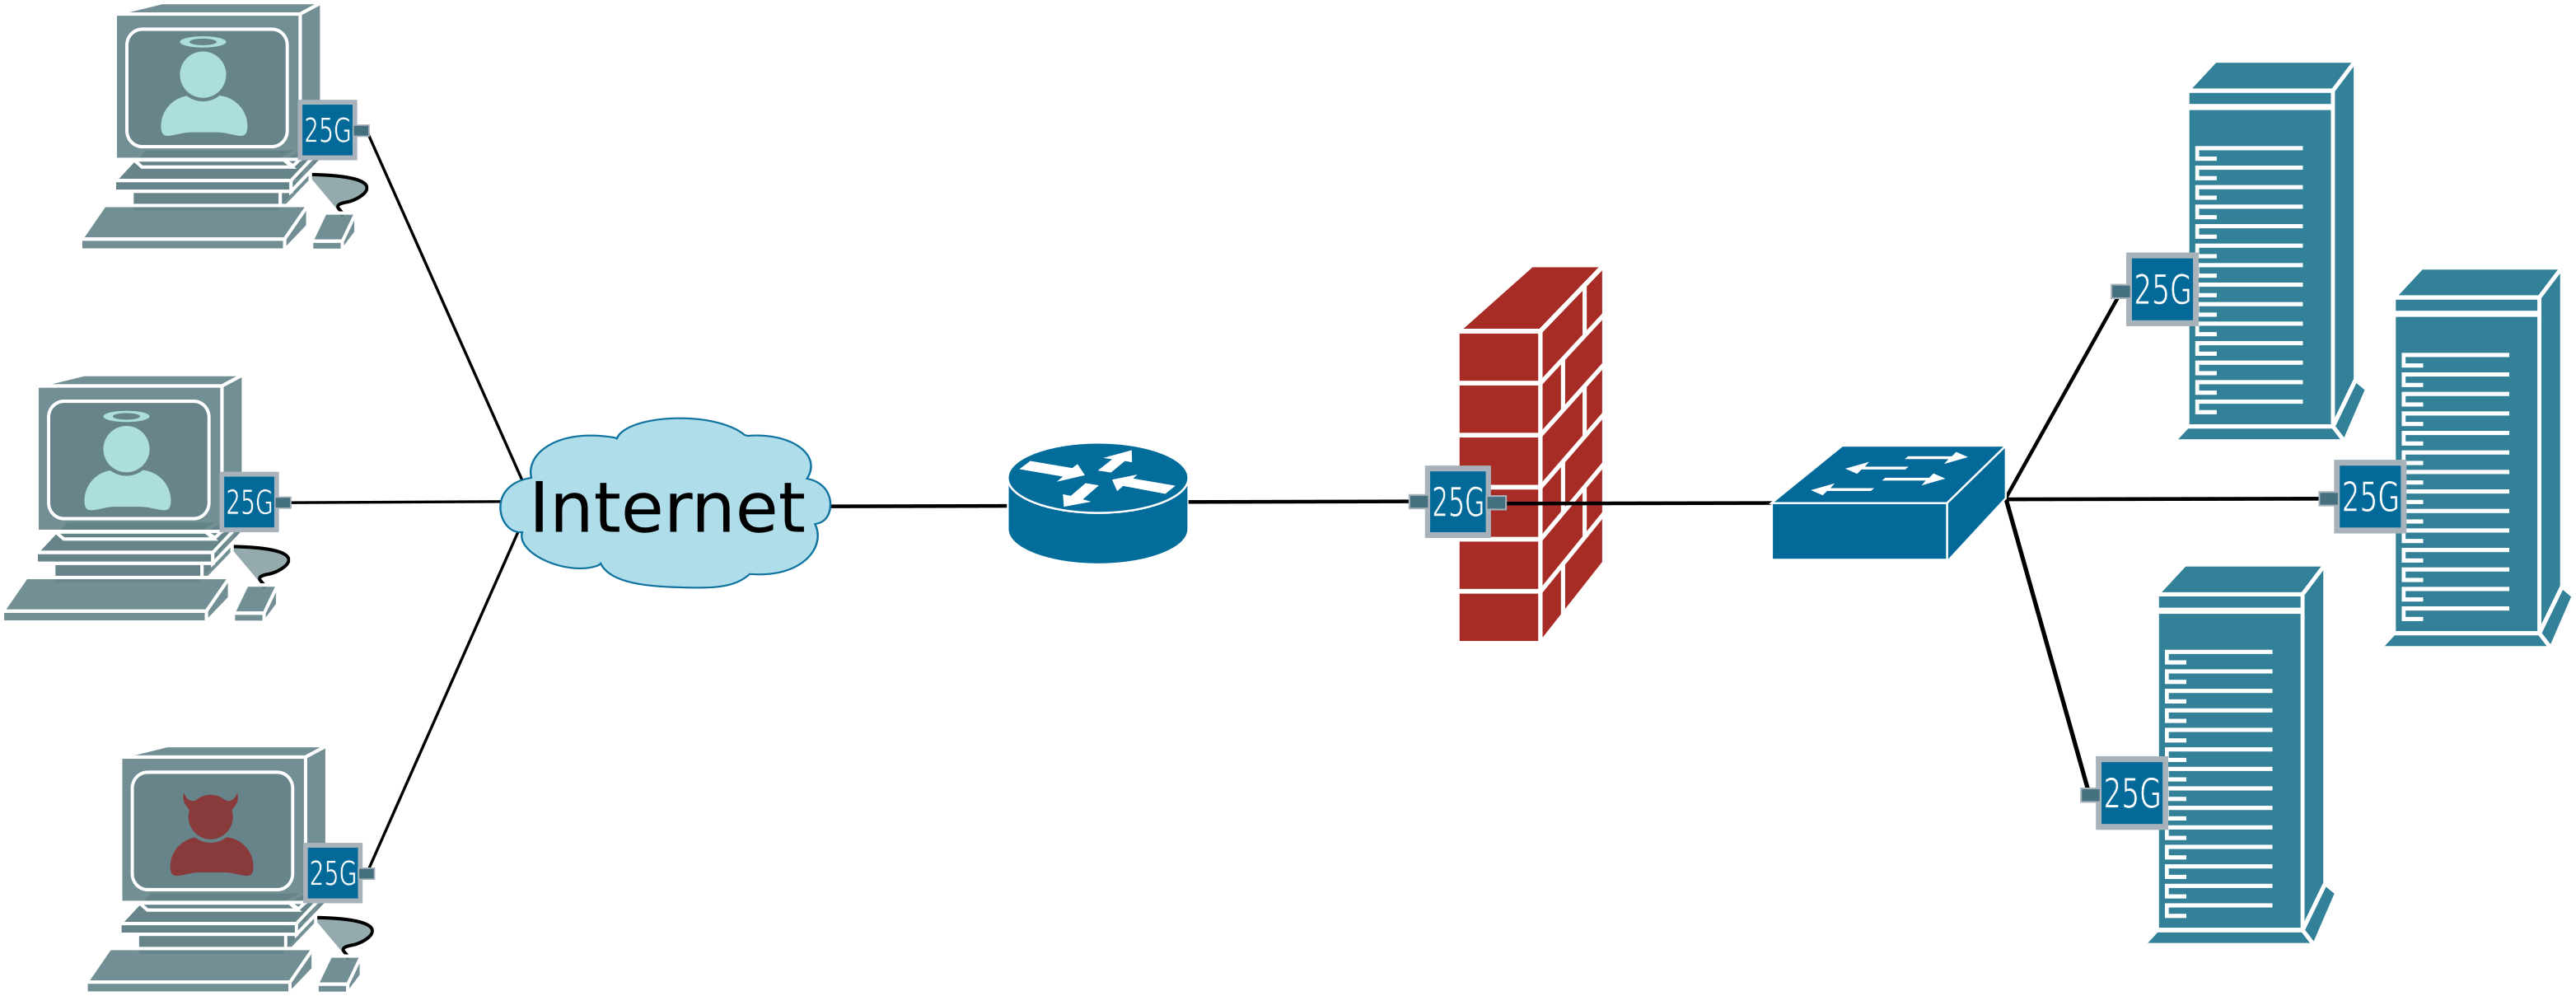
\includegraphics[width=1.0\linewidth]{Netzwerkplan-Real}
    \caption{Realaufbau unter Verwendung eines Angreifers}
    \label{fig:netzwerkplan-real}
\end{figure}
\begin{figure}[t]
	\centering
	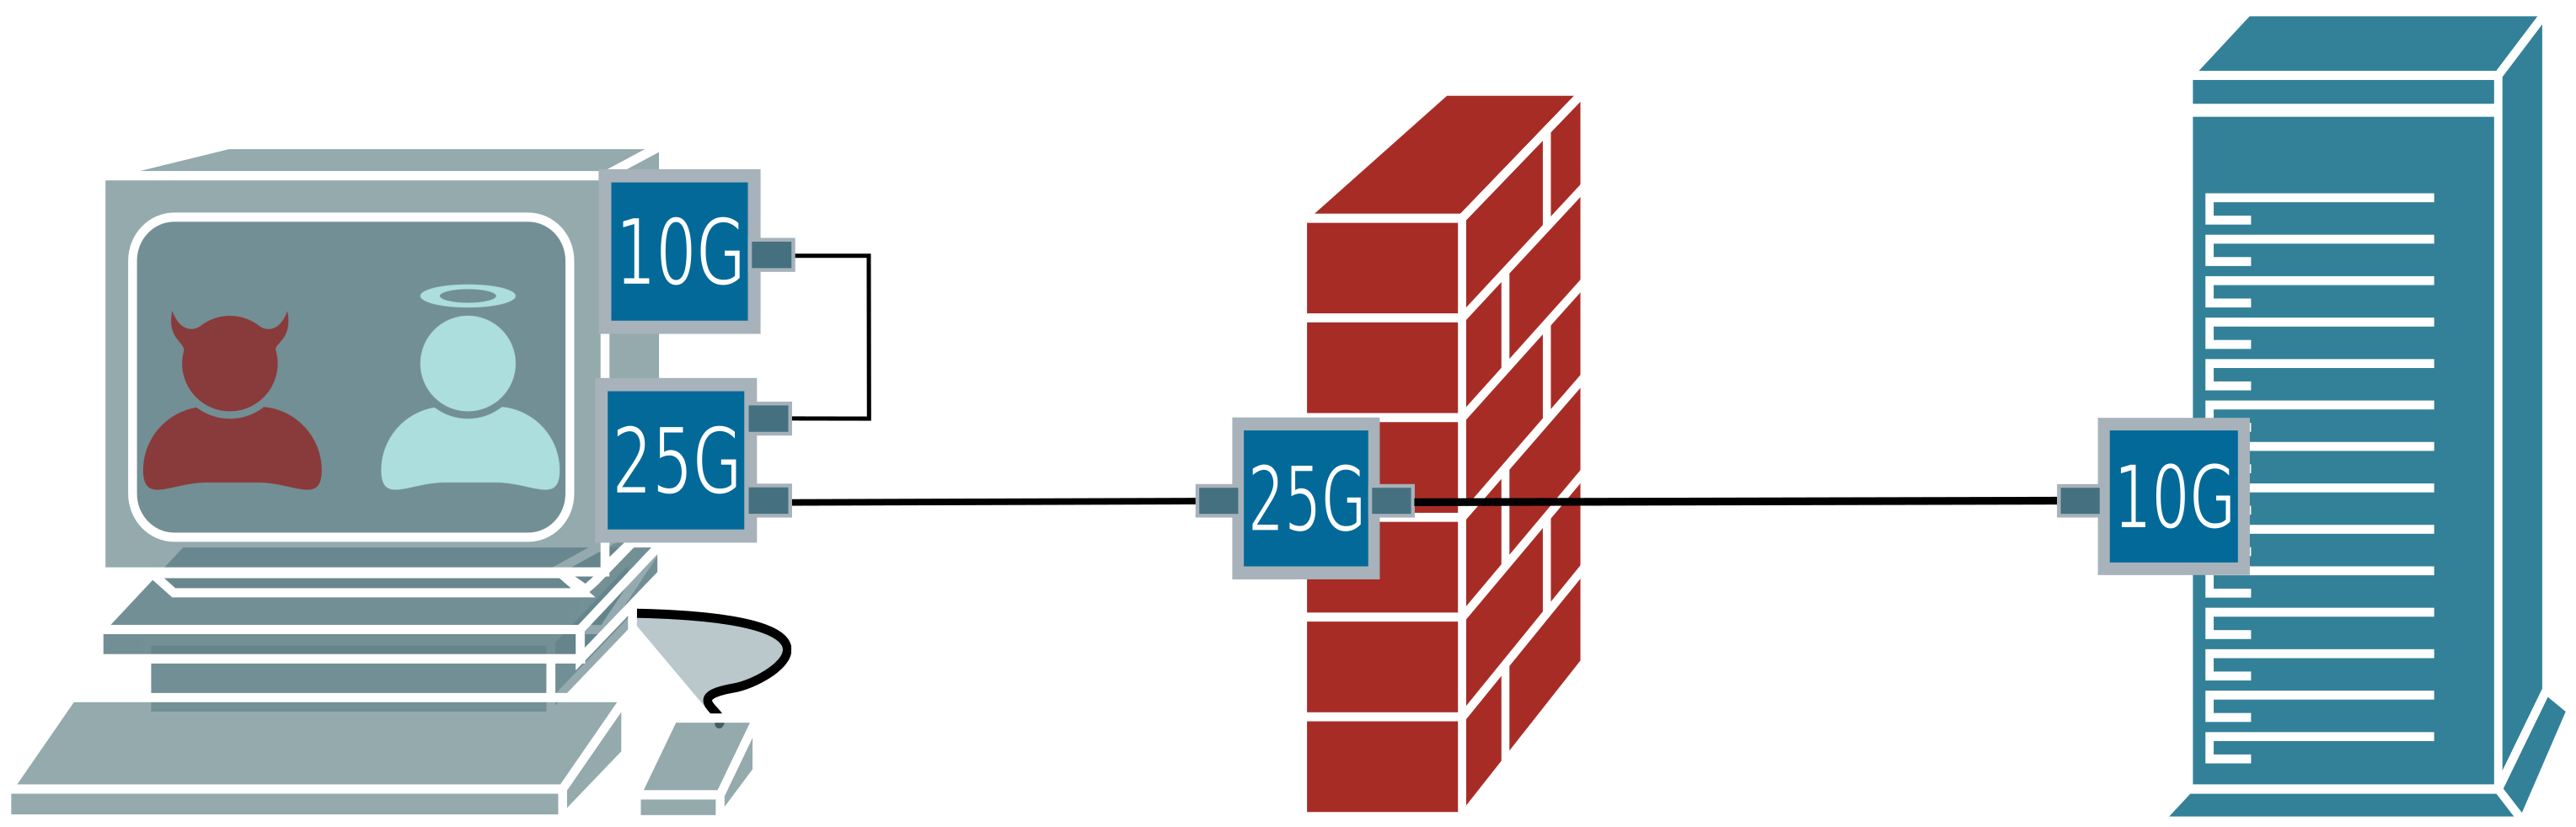
\includegraphics[width=0.6\linewidth]{Netwerkplan-Versuch}
	\caption{Versuchsaufbau}
	\label{fig:Versuchsaufbau}
\end{figure}

\section{Angriffsvarianten und Abwehrmechanismen}
Das zu entwickelnde System muss Schutz bieten, gegen die bereits in der Analyse erwähnten Angriffe. Hierunter fallen die SYN-Flut, der SYN-FIN beziehungsweise SYN-FIN-ACK Angriff, sowie die beiden Ausformungen des Sockstress, TCP Small- und TCP Zero-Window. Des weiteren muss Schutz gegen die UDP Flut geboten werden.

Zur Verhinderung der Angriffe ist im Aufbau \ref{fig:Versuchsaufbau} vorgesehen, dass sich eine Middlebox zwischen dem zu schützenden System und dem externen Netz befindet. Um einen effektiven Schutz gegen oben genannte Angriffe bieten zu können, wird eine Inspektion der Verbindungsströme zum Einsatz kommen. Prinzipiell ist vorgesehen, dass die Middlebox alle gesendeten Pakete abfängt, inspiziert, klassifiziert und bei Erkennung von Angriffen auf diese reagiert, sowie legitimen Verkehr an die entsprechenden Server und Nutzer weiterleitet. Die Detektion und Klassifizierung geschieht dabei individuell nach Angriffsmuster.

\subsection{SYN-FIN und SYN-FIN-ACK Attacke}
\begin{figure}[t]
    \centering
    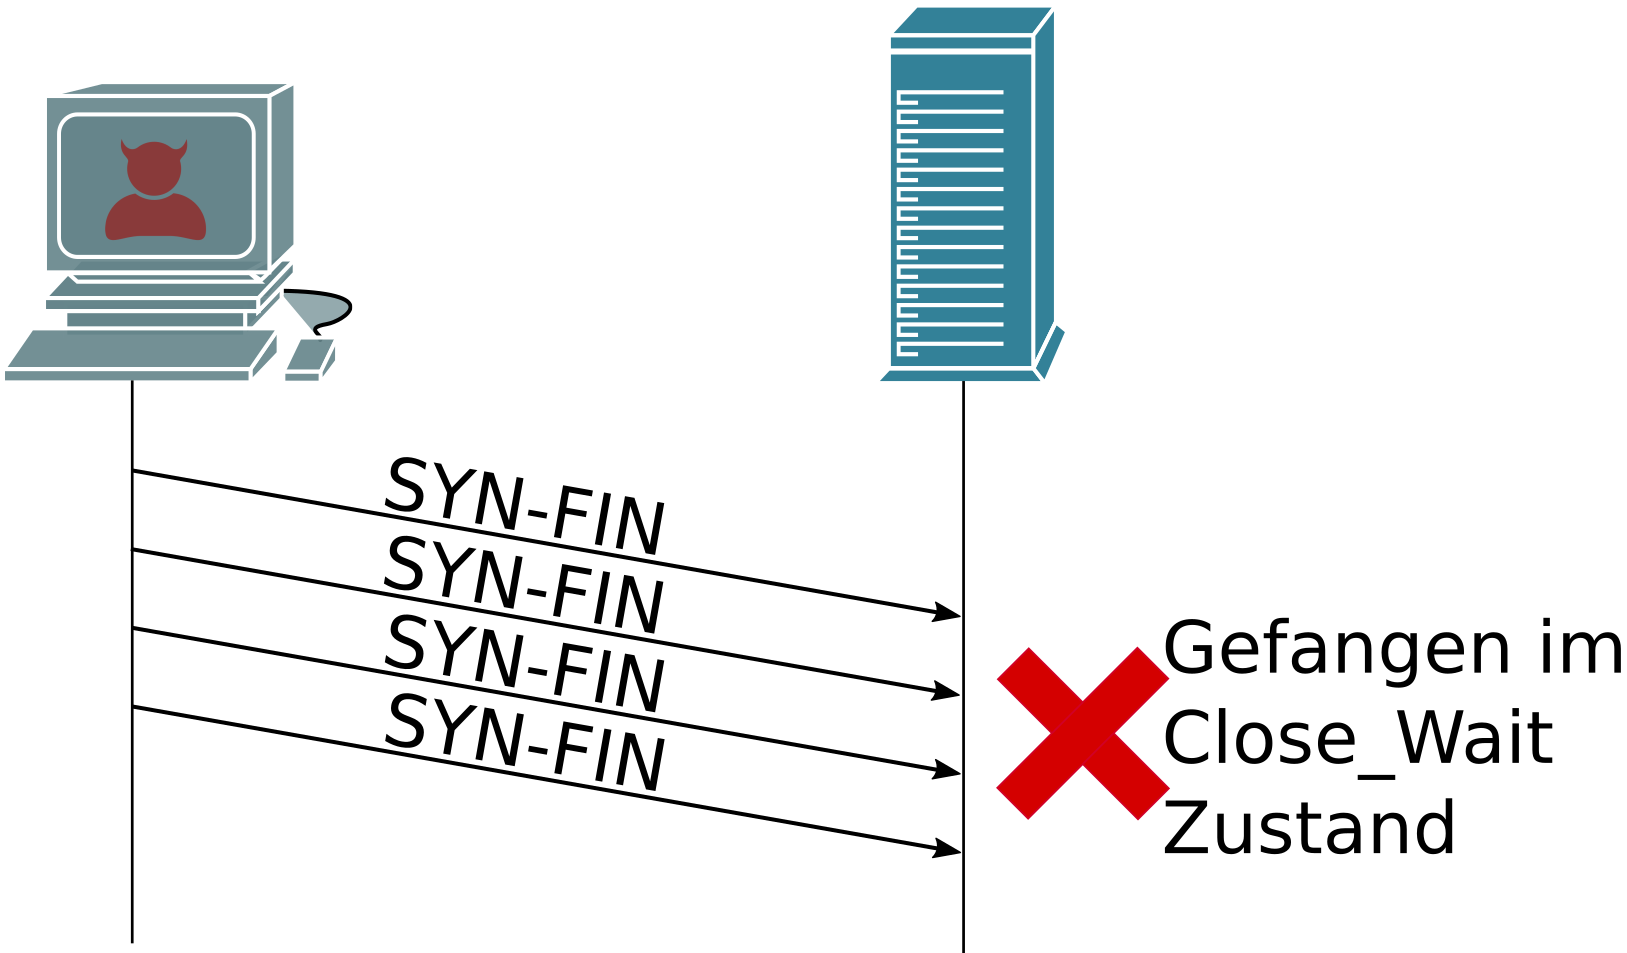
\includegraphics[width=0.5\linewidth]{SYN-FIN}
    \caption{Schematische Darstellung der SYN-FIN Attacke}
    \label{fig:SYN-FIN}
\end{figure}

Eine SYN-FIN-(ACK) Attacke zeichnet sich dadurch aus, dass ein Angreifer, oftmals in Form eines Botnets, in Abbildung \ref{fig:SYN-FIN} auf der rechten Seite zu sehen, unablässig TCP Pakete mit gesetztem SYN und FIN Flag an das Opfer schickt. In Folge dessen ist es möglich, dass der Server in einem Close\_Wait Zustand gefangen ist, und in Folge dessen betriebsunfähig wird.

Zur Erkennung einer SYN-FIN sowie SYN-FIN-ACK Attacke werden die gesetzten TCP Flags verwendet, sobald in einem TCP Paket sowohl SYN als auch FIN oder in zweitem Fall zusätzlich noch das ACK-Flag gesetzt sind, klassifiziert die Software das Paket als verdächtig und verwerfen dieses in Folge der Abwehrstrategie.

Abbildung \ref{fig:seqsynfinack} zeigt den wohl einfachsten Ablauf einer Abwehrstrategie, bei der SYN-FIN-(ACK) Attacke reicht der Analyzer selbst aus um die Abwehr zu realisieren. Zuerst erhält der Analyzer die Paketinfos in Form eines rte\_ring Pointers, es folgt die Detektion des Angriffs, sobald ein Paket erkannt wurde, welches die Angriffscharakteristika aufweist, wird dieses gedroppt.

\subsection{SYN-Flut}
\begin{figure}[t]
    \centering
    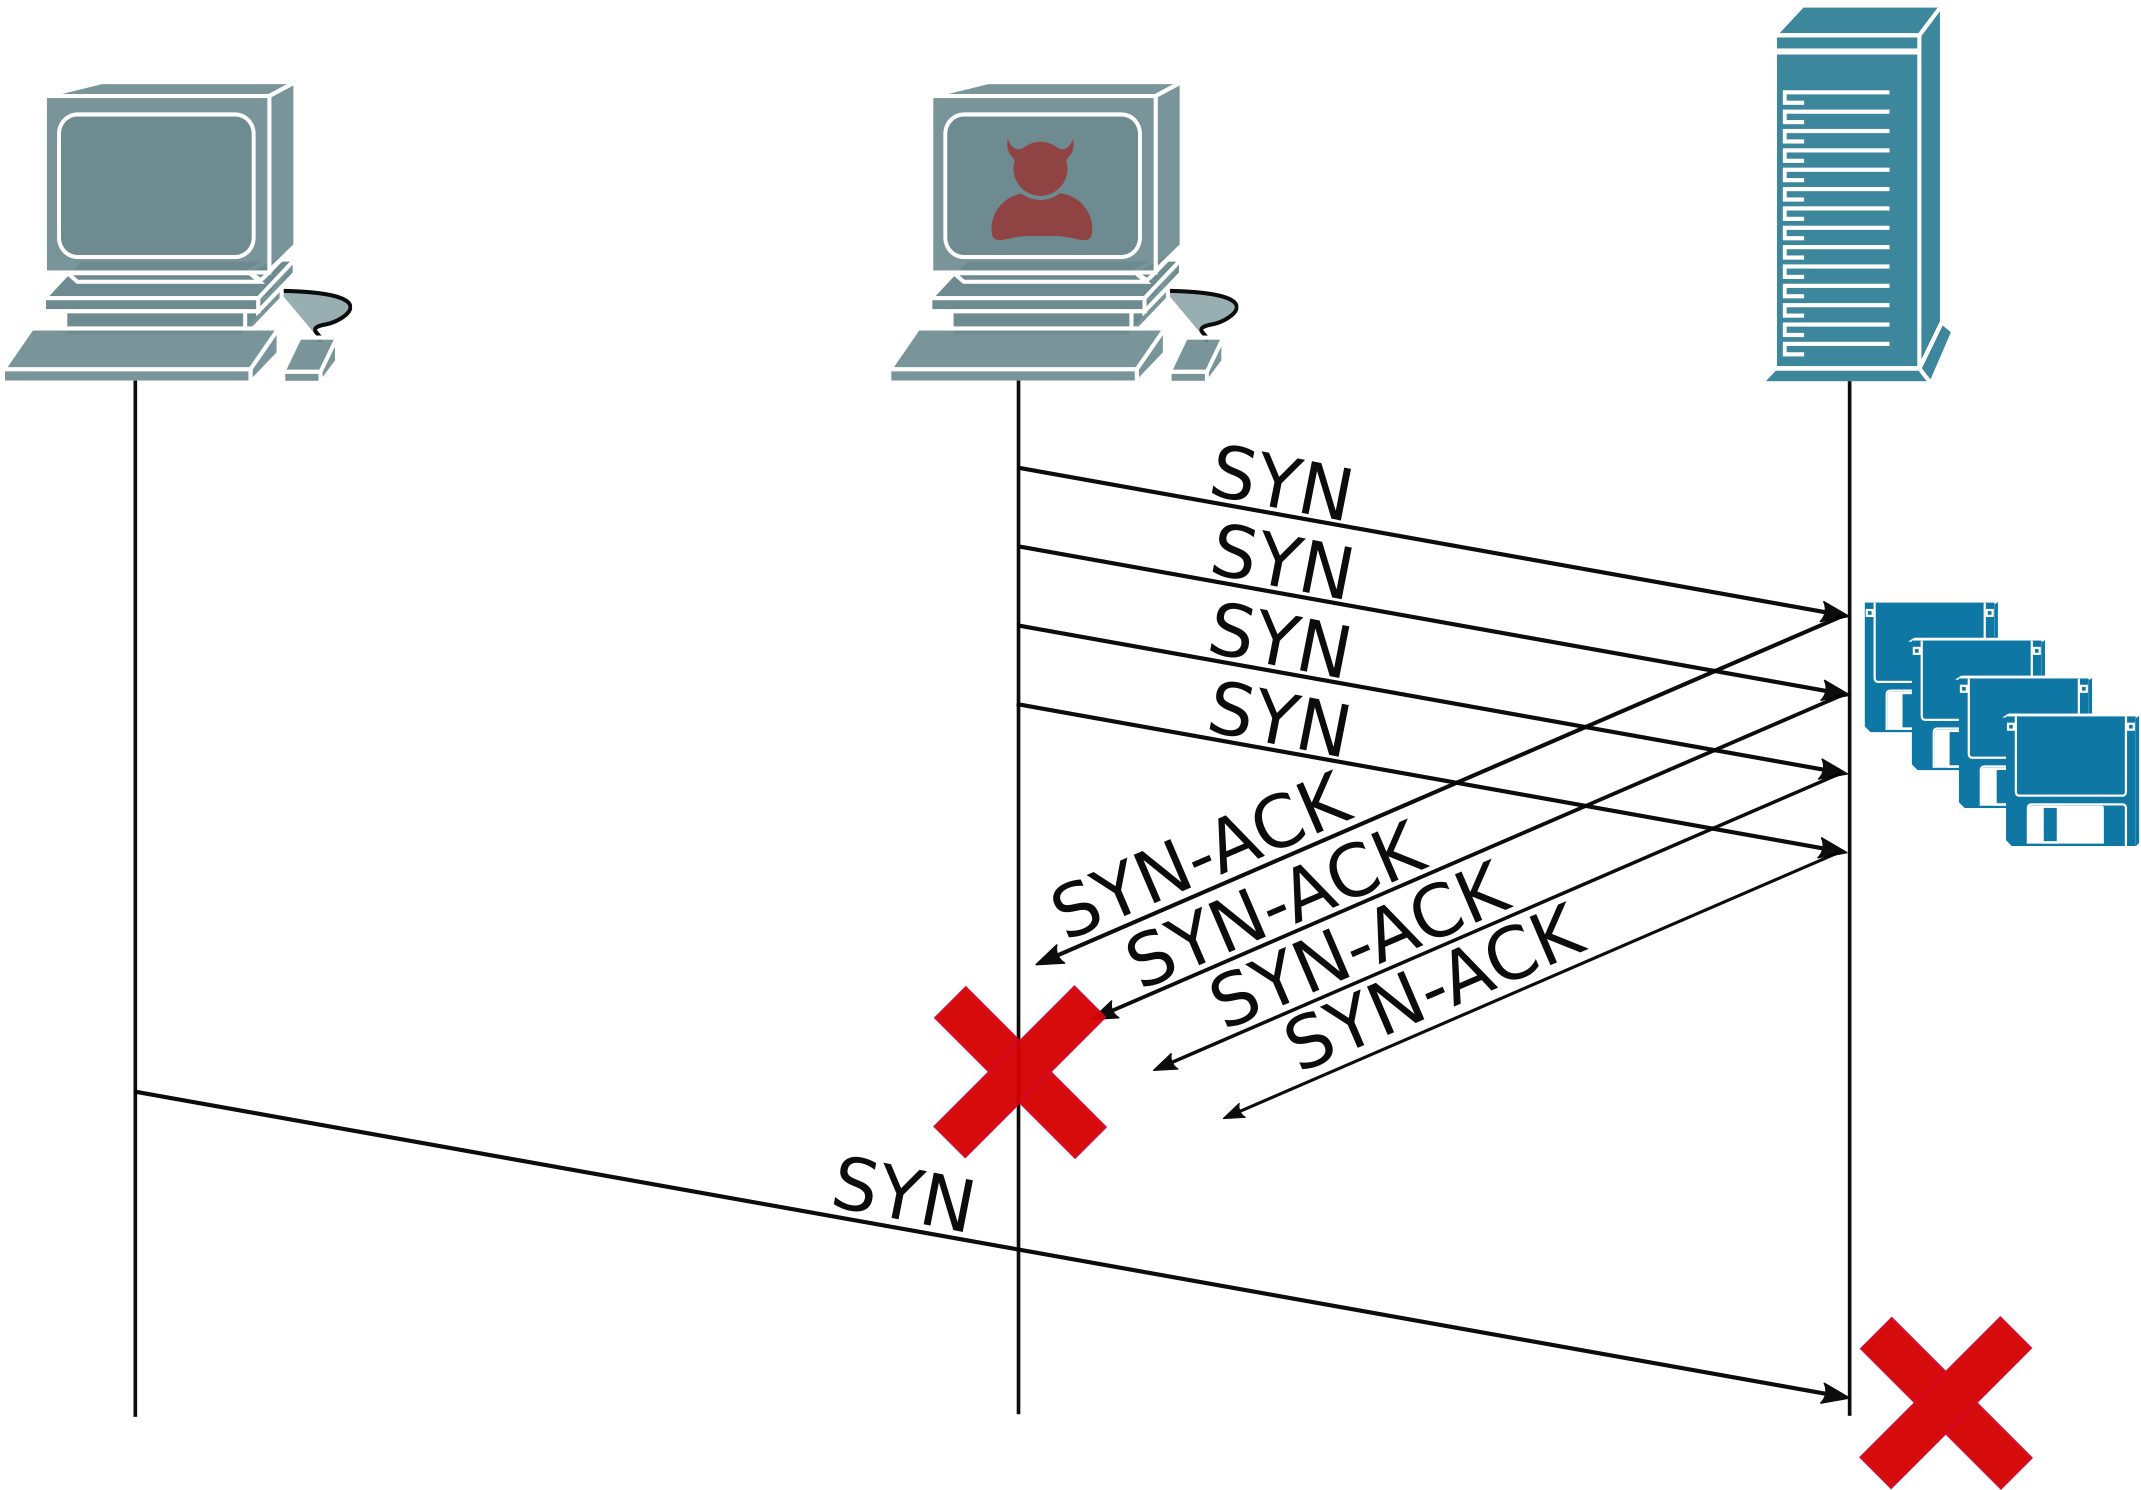
\includegraphics[width=0.5\linewidth]{SYN-Flood}
    \caption{Schematische Darstellung der SYN-Flut Attacke}
    \label{fig:SYN-Flood}
\end{figure}

Eine SYN-Flut Attacke läuft prinzipiell wie folgt ab. Der Angreifer, in Abbildung \ref{fig:SYN-Flood} mittig dargestellt, schickt viele TCP Pakete mit gesetztem SYN-Flag an das Opfer, und bekundet somit den Wunsch eine Verbindung aufzubauen. Der Server antwortet mit TCP Pakten mit gesetzten SYN-ACK Flags und speichert erste Informationen über die sich im Aufbau befindende Verbindung, welche allerdings aufgrund von gefälschten IP Absenderadressen oder einer Verwerfstrategie am Angriffsrechner nie mit dem vom Server erwarteten TCP Paket mit ACK Flag beantwortet wird. Der Server hält also Informationen für Verbindungen vor, welche nie korrekt aufgebaut wurden und werden. Dies führt im schlechtesten Fall zu abgelehnten Verbindungen von legitimen Nutzern oder einem Totalausfall des Servers.

Die Erkennung einer SYN-Flut beruht auf der Zählung der eingehenden TCP Pakete, welche das SYN-Flag gesetzt haben, den ausgehenden Paketen, welche das SYN und ACK Flag gesetzt haben, sowie der Anzahl an zu den Verbindungsaufbauanfragen gehörenden ACKs, also den letztendlich gelungenen Verbindungsaufbauten.

Um einer SYN-Flut standzuhalten, setzt das zu entwickelnde System auf die Verwendung von SYN-Cookies, hierbei speichert die Middlebox keine Informationen über halboffene Verbindungen, sondern lagert diese Informationen in den Paketheader aus. Die Sequenznummer eines Paketes enthält nun das Ergebnis einer Hashfunktion, welche die Informationen, welche vorher gespeichert waren, kodiert. Dies beschreibt wie sich die Middlebox selbst vor einer SYN-Flut schützt. Um allerdings die dahinterliegenden Server zu schützen, übernimmt die Middlebox auch eine weitere Funktion. Sie baut für alle zu schützenden Systeme die TCP Verbindungen mit externen Hosts auf, sobald dies erfolgreich geschehen ist, wird durch das zu entwickelnde System eine weitere Verbindung mit dem Zielrecher des ursprünglich von außen ankommenden Pakets auf, und leitet fortan Pakete von der externen Verbindung an die Interne weiter. Dies geschieht unter anderem durch eine Anpassung von Sequenznummern mittels eines verbindungsspezifischen Offsets, nicht zu vergessen ist hierbei die Anpassung der Checksumme und anderer Headerfelder.

Abbildung \ref{fig:SYN-Flood-Abwehr} soll den geplanten Aufbau nochmals verdeutlichen und insbesondere zum besseren Verständnis des Sequenznummermappings beitragen. Wie in der Abbildung angedeutet, findet zuerst ein Verbindungsaufbau zwischen Middlebox und externem System statt, sobald die Middlebox ein passendes ACK vom externen Nutzer erhalten hat, wird von der Middlebox eine Verbindung zum eigentlichen Ziel aufgebaut. In Folge dessen muss nun für jedes nachfolgende Paket, unabhängig davon, ob dieses von Innen nach Außen oder umgekehrt geschickt wird, eine Anpassung der Sequenznummern vorgenommen werden. Anzumerken ist hierbei, dass in Abbildung \ref{fig:SYN-Flood-Abwehr}, die Payload X als Anfrage, und die Payload Y als Antwort hierauf zu verstehen ist.
\begin{figure}[t]
    \centering
    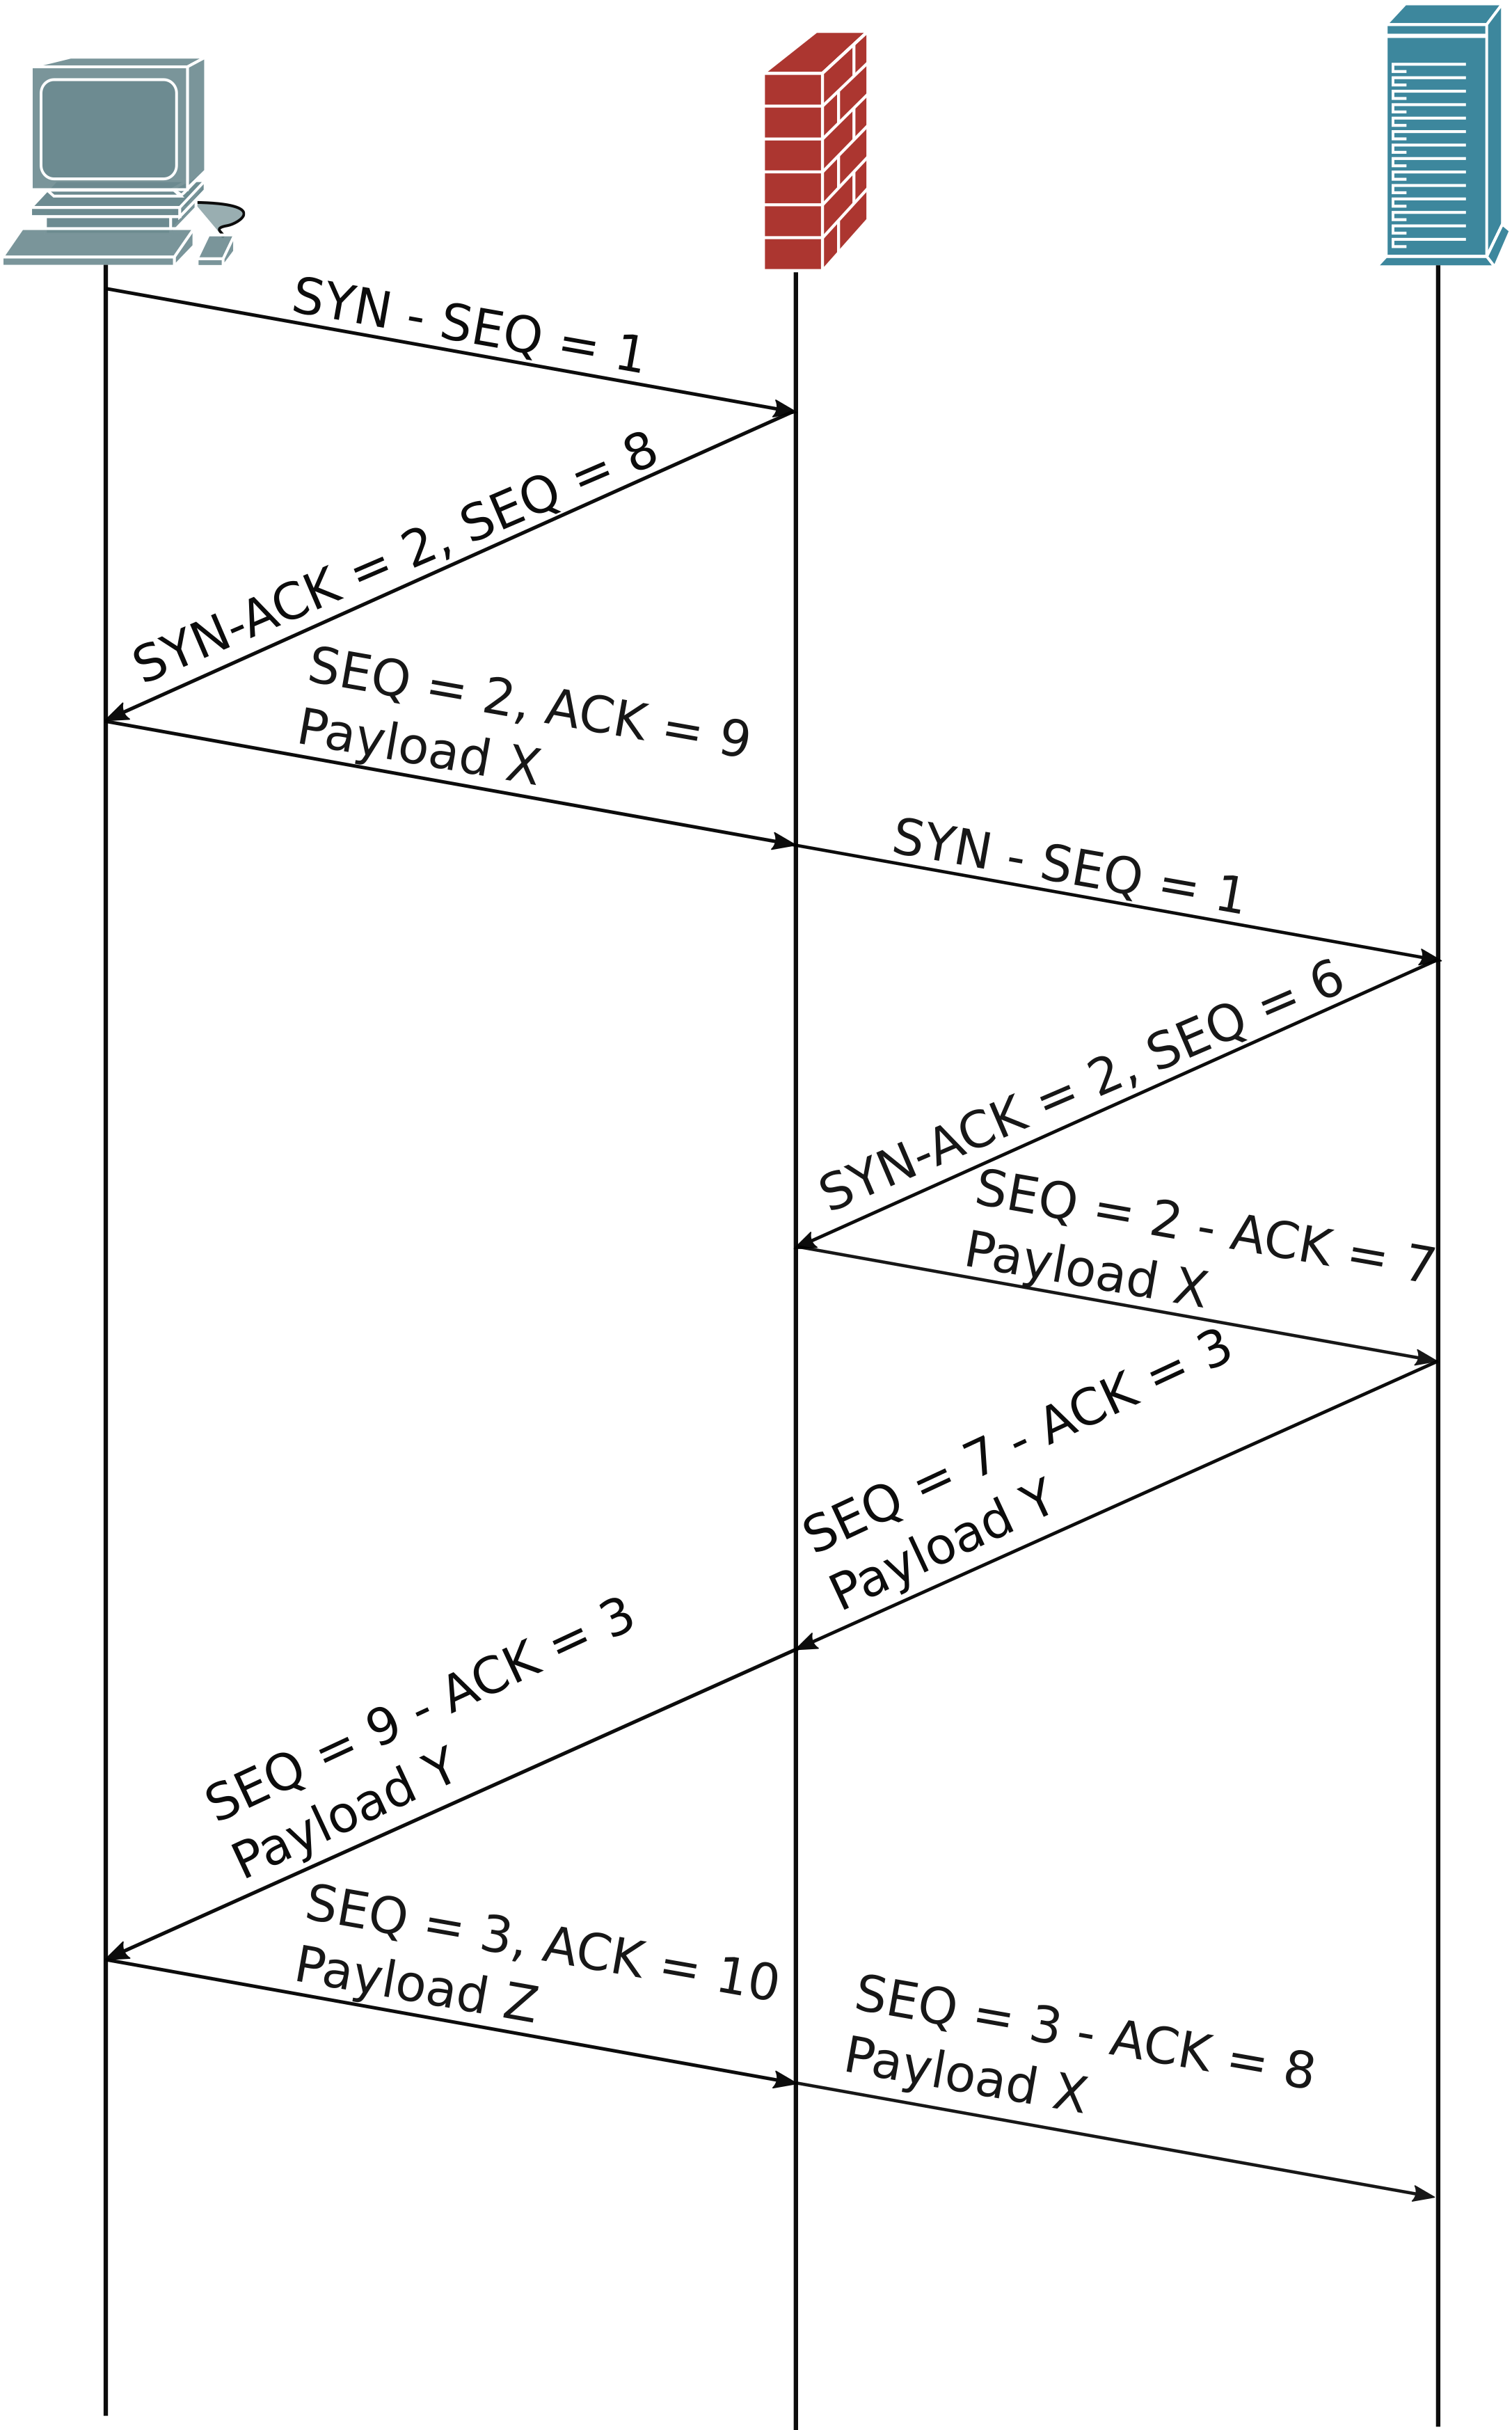
\includegraphics[width=0.5\linewidth]{SYN-Flood-Abwehr}
    \caption{Schematische Darstellung des Abwehr der SYN-Flood}
    \label{fig:SYN-Flood-Abwehr}
\end{figure}

% Sollte die Kombination aus diesen beiden Verhinderungsstrategien widererwartens nicht ausreichend sein, wäre auch eine zusätzliche SYN-Authentication denkbar 

\subsection{Zero-Window}
\begin{figure}[t]
    \centering
    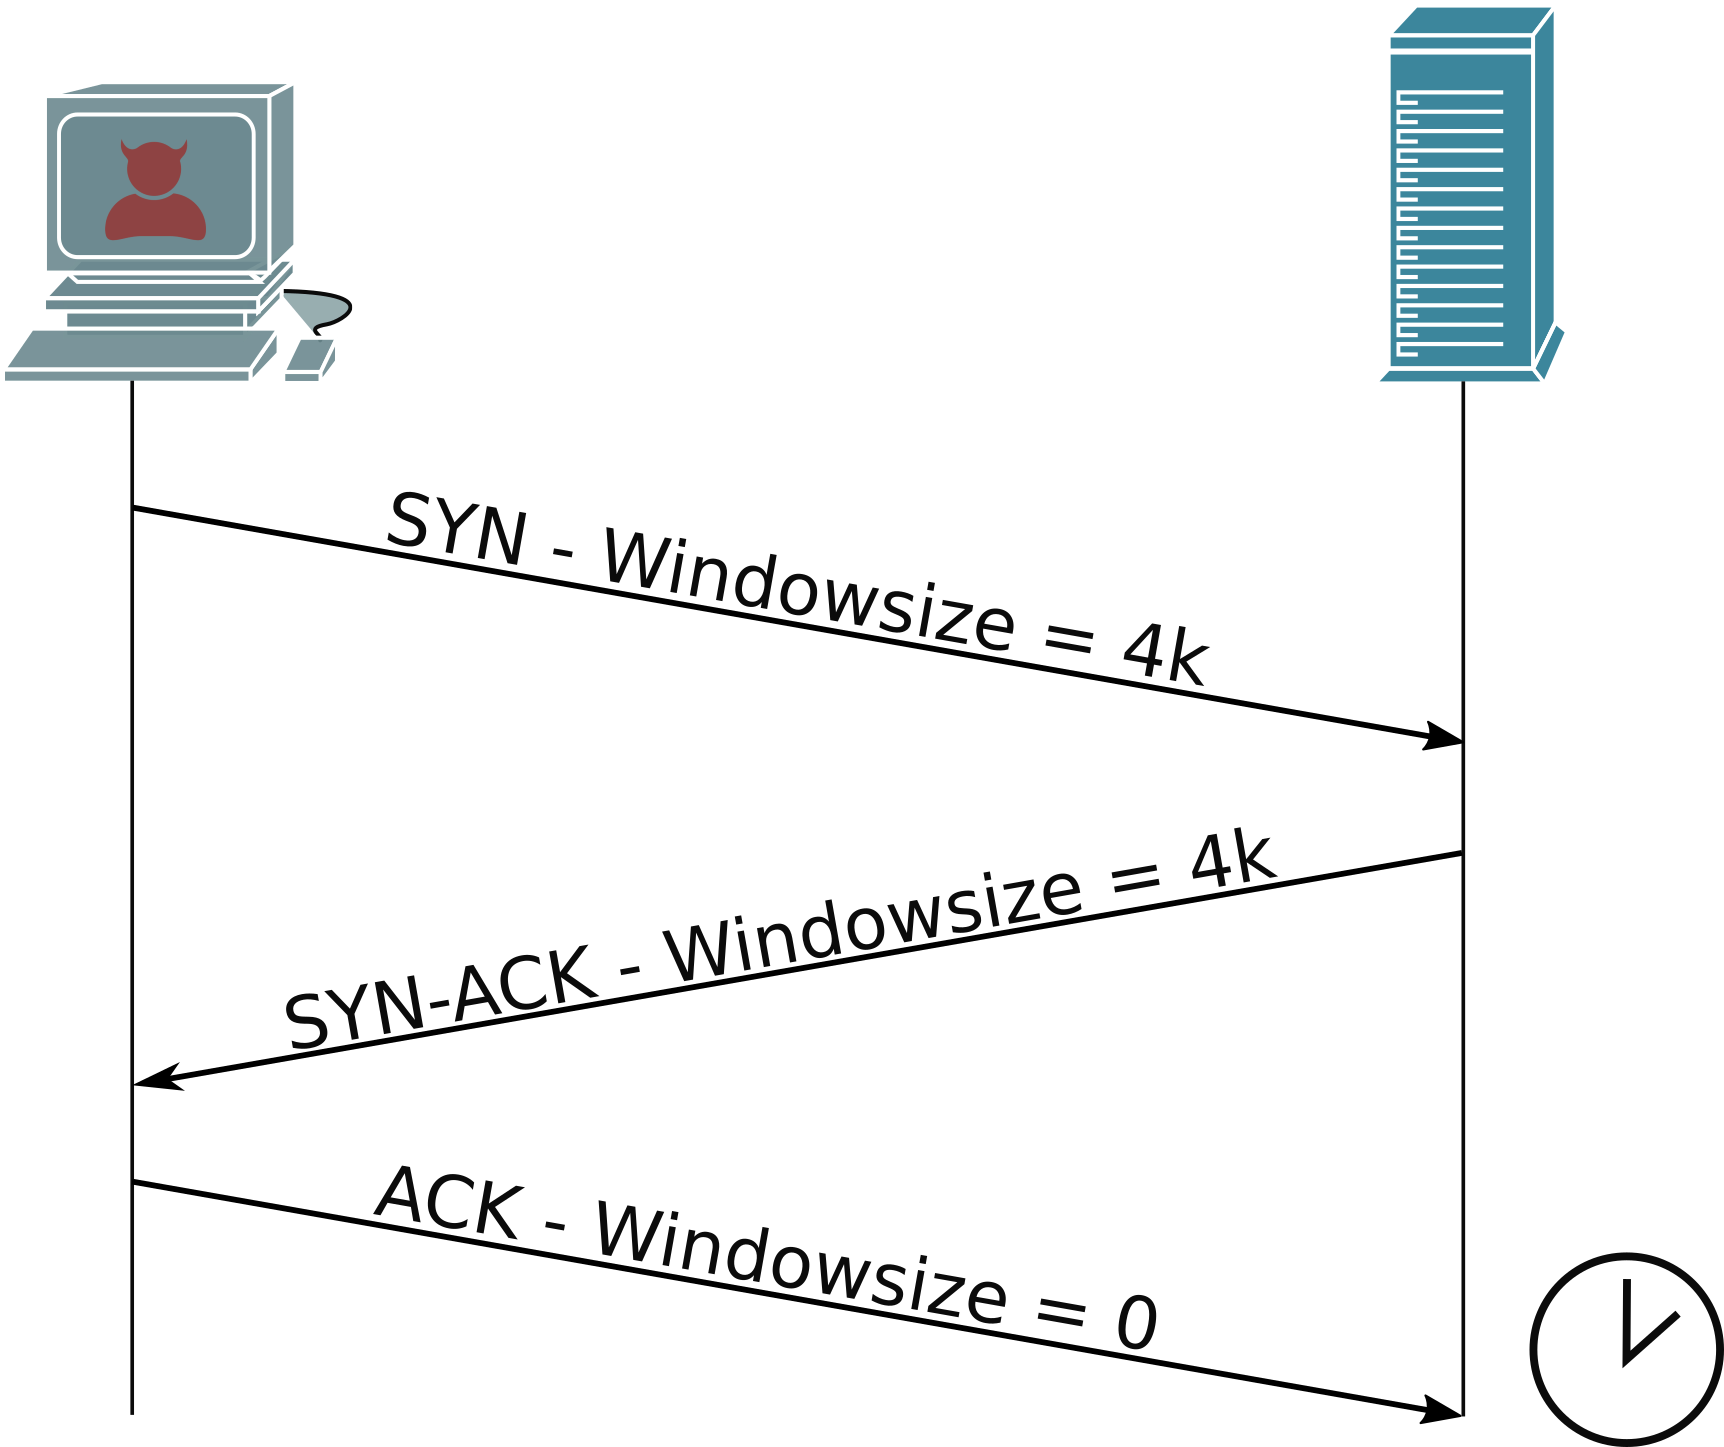
\includegraphics[width=0.5\linewidth]{Zero-Window}
    \caption{Schematische Darstellung der Zero-Window Attacke}
    \label{fig:Zero-Window}
\end{figure}
Die TCP-Zero-Window Attacke, siehe Abbildung \ref{fig:Zero-Window} beruht darauf, dass ein Angreifer mehrere Verbindungen zu einem Opferserver aufbaut, und sein Empfangsfenster auf Größe 0 setzt. Somit werden auf dem Server Ressourcen für eine Verbindung verbraucht, welche keinen legitimen Zweck hat.
Werden sehr viele solcher Verbindungen aufgebaut, kann es gar geschehen, dass ein Server keinerlei legitime Verbindungen mehr aufbauen kann. Allerdings kann es auch in legitimen Verbindungen kurzzeitig dazu kommen, dass das Empfangsfenster des Nutzers auf die Größe null gesetzt wird.

Um die TCP Zero Window Attacke zu erkennen, wird unter Anderem die Zählung aller Verbindungen, welche ein Zero-Window ankündigen, verwendet. Da dies alleine allerdings zur Erkennung nicht ausreichend ist, muss eine zeitliche Statistik über diese Verbindungen geführt werden. Sobald eine TCP Verbindung über einen gewissen Zeitraum ein Zero-Window ankündigt und dies nie verändert, wird die Verbindung als auffällig erkannt. Bei genauerer Kenntnis der zu schützenden Systeme wäre es ebenfalls möglich zu zählen, wie viele TCP-Verbindungen zu einem gewissen System mit Fenstergröße null aufgebaut sind. Hierdurch könnte nun bei Kenntnis der maximal erlaubten konkurrierenden Verbindungen eines Webservers, errechnet werden, ob die Anzahl der Verbindungen mit Fenstergröße null einen kritischen Anteil erreicht. Als Lösungsstrategie ist hier ein Timeout für TCP-Verbindungen mit Fenstergröße 0 vorgesehen, sowie eine Ratenbegrenzung von TCP-Verbindungen pro Zielsystem.
\subsection{Small-Window}
\begin{figure}[t]
    \centering
    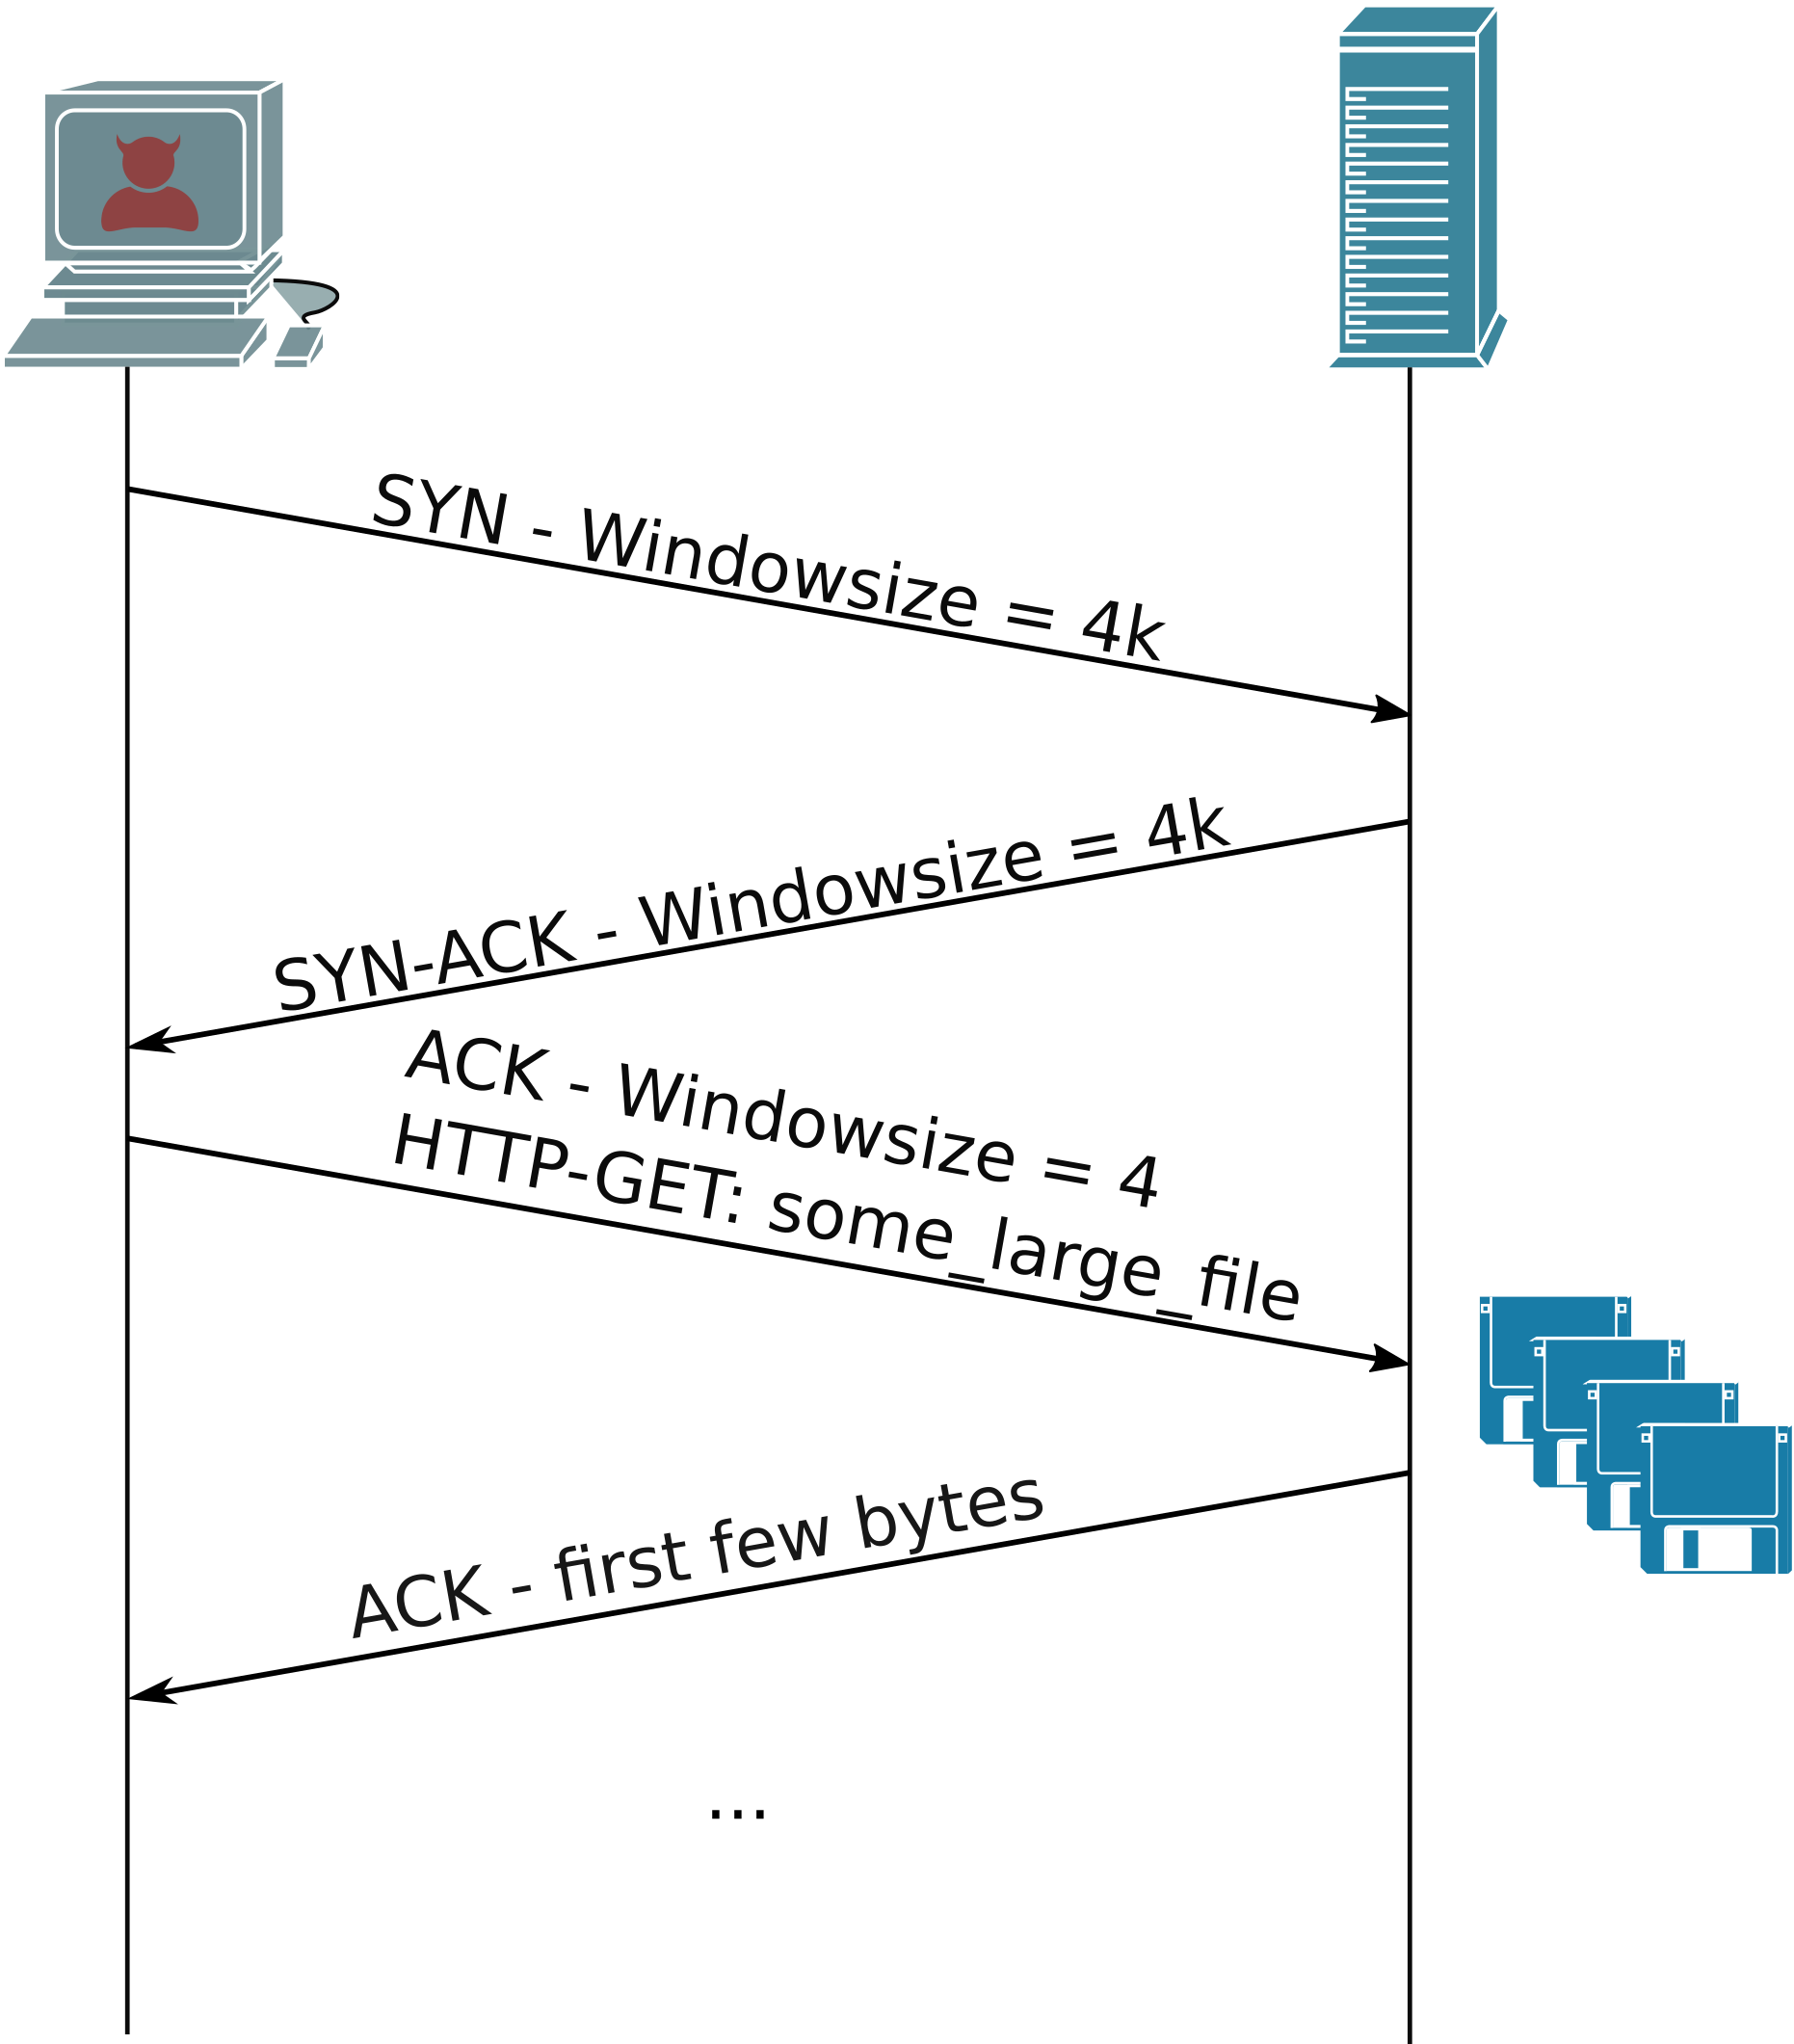
\includegraphics[width=0.55\linewidth]{Small-Window}
    \caption{Schematische Darstellung der Small-Window Attacke}
    \label{fig:Small-Window}
\end{figure}
Ein TCP-Small Window Angriff, siehe \ref{fig:Small-Window} beruht prinzipiell darauf, das  ein Angreifer eine TCP Verbindung zu einem Server aufbaut und direkt eine sehr große Datei anfordert. Hierbei setzt der Angreifer gleichzeitig sein Empfangsfenster auf eine sehr kleine Größe, sodass der sendende Server die angeforderte Ressource zuvor in viele kleine Fragmente aufteilen muss. Dies kostet nicht nur Speicherplatz, sondern auch Rechenleistung. Als Resultat ist es möglich, dass der Server Speicherüberläufe erleidet und gänzlich abstürzt.

Die Erkennungsstrategie von TCP Small Window stellt sich als schwieriger zu Realisieren dar, hier sind bislang verschiedene Optionen im Gespräch. Eine Auffälligkeit, welche ein Angreifer aber leicht umgehen könnte, sind der konstante Einsatz von nur einer Fenstergröße. Unter Umständen lässt sich die Erkennung noch verbessern, wenn das zu entwerfende System eine Übersicht über alle abrufbaren Ressourcen der zu schützenden Systeme besitzt.
Die Verhinderung oder Abschwächung von TCP Small Window Angriffen beruht auf dem Setzen eines absoluten Verbindungstimeout, dessen Wert sich an der mittleren Verbindungsdauer für diesen Server oder dieses Netzwerk orientiert. Um den Schutz noch effektiver zu gestalten wird des Weiteren eine minimale, nicht zu unterschreitende Datenrate definiert. Fallen mehrere Verbindung unter diese Rate, so sind die ältesten als nicht legitim zu erachten und zu beenden.

\subsection{UDP-Flood}
\begin{figure}[t]
    \centering
    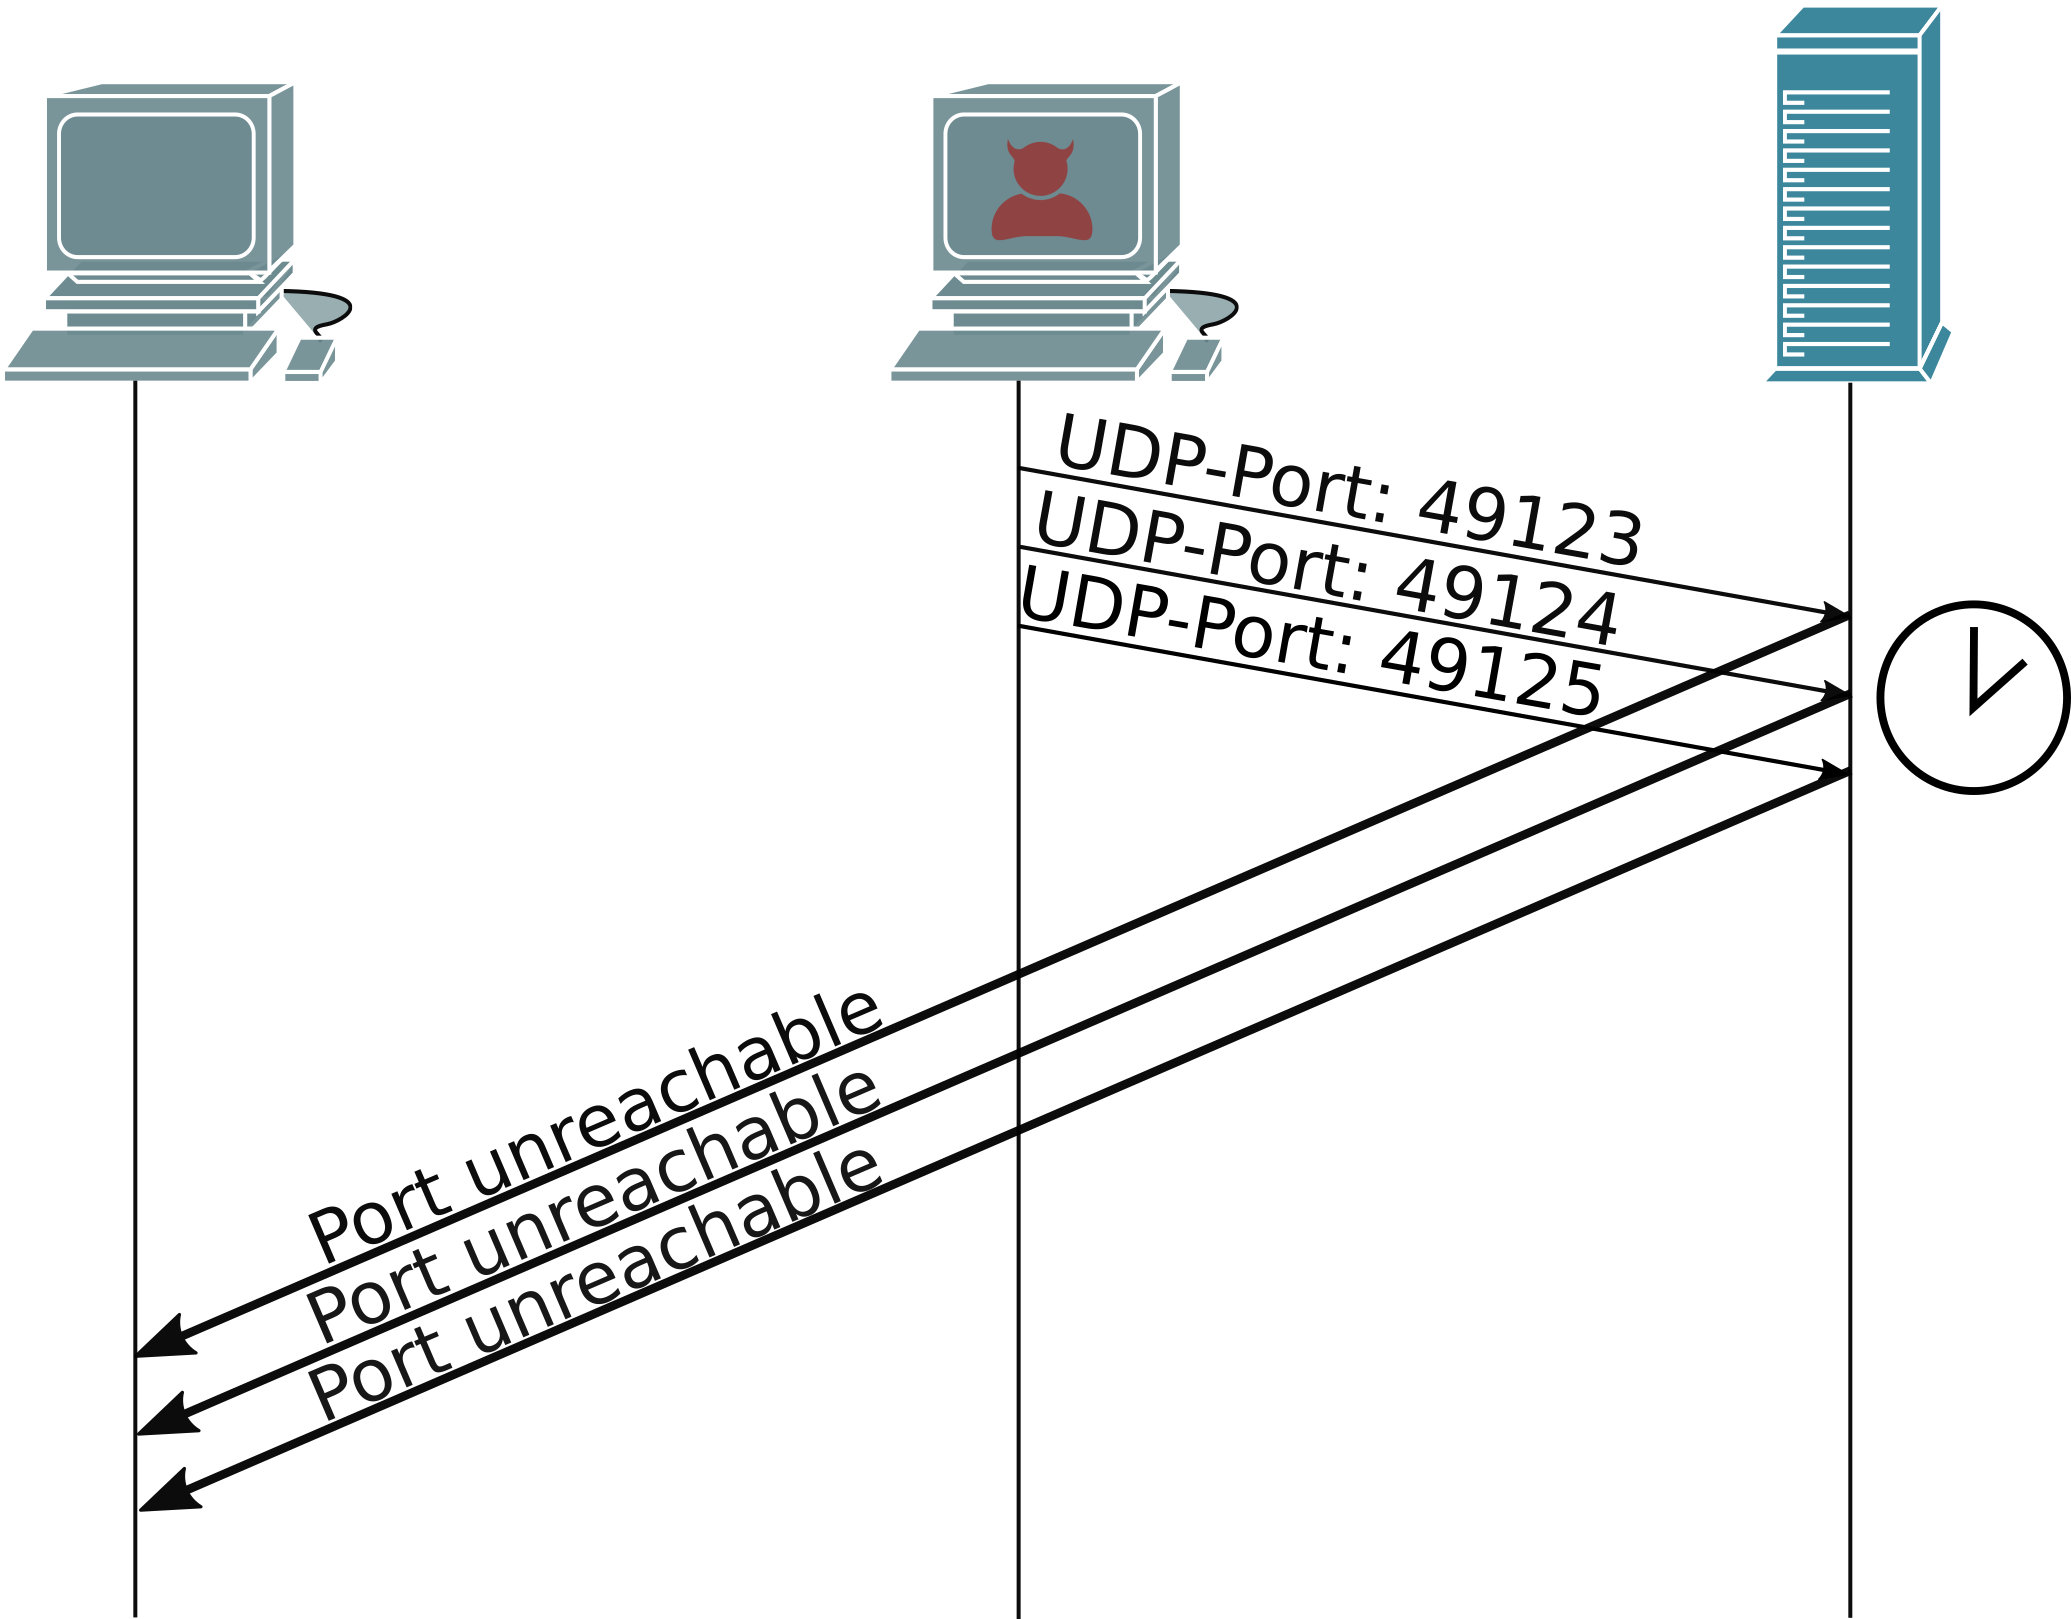
\includegraphics[width=0.55\linewidth]{UDP-Flood}
    \caption{Schematische Darstellung der UDP-Flood}
    \label{fig:UDP-Flood}
\end{figure}

Die UDP-Flut, siehe Abbildung \ref{fig:UDP-Flood}, zeichnet sich durch eine hohe Anzahl an UDP-Nachrichten an einzelne Zielsysteme aus. Für jede Nachricht prüft das Opfersystem, ob gerade eine Anwendung auf diesem Port lauscht, ist dies nicht der Fall, so reagiert es mit Port unreachable Nachrichten. Die Überprüfung und der Versand dieser Nachrichten benötigt Rechenleistung und Zeit. Im schlechtesten Fall wird durch diesen Angriff der Verkehr komplett zum Erliegen gebracht.

Zur Erkennung dieser würde auf die Verbindungsstatistik, welche darstellt, auf welchen Zielrechnern vermehrt Ports angefragt werden, gesetzt. Wird bei einem zu schützenden Server eine fest definierte Abfragerate überschritten, würde das System eine UDP Flood erkennen. Da dies allerdings im angestrebten Abwehrszenario nicht benötigt wird, um den Angriff abzuwehren, findet im System diese Erkennung ausschließlich zu statistischen Zwecken statt. Um die UDP-Flut allerdings erfolgreich Abwehren zu können, setzt das System auf eine Ratenlimitierung für UDP Traffic pro zu schützendem System.
%\subsection{Zusätzlich} %TODO
%Im Allgemeinen wäre es in diesem System unter Umständen auch sinnvoll, White- und Blacklists einzusetzen, welche gewissen externen IPs Zugriff gestatten oder komplett verweigern. Um den Rechenaufwand auf dem System zu verringern, wäre es auch von Vorteil diese Listen, mit der Möglichkeit IPs temporär in solche einzutragen, zu gestalten.

% !TODO
% Ziel 
% - 25Gbps = $\frac{25*10^9 \frac{bit}{sec}}{(64 +20,2)*8 bit}$  = 37.1 Mpps
% - pro Paket $2.7^{-8}$ Sekunden Verarbeitungszeit
\section{Grundlegender Aufbau der Software} \label{section:basic_structure}
Das Grundprinzip der zu entwickelten Software soll sein, Pakete auf einem Port der Netzwerkkarte zu empfangen und diese zu einem anderen Port weiterzuleiten. Zwischen diesen beiden Schritten werden die Pakete untersucht, Daten aus diesen extrahiert und ausgewertet. Im weiteren Verlauf des Programms werden Pakete, welche einem Angriff zugeordnet werden verworfen, und legtime Pakete zwischen dem interen und externen Netz ausgetauscht. Es bietet sich an, hier ein Pipelinemodell zu verwenden wobei die einzelnen Softwarekomponenten in Pakete aufgeteilt werden. Im ConfigurationManagement werden die initialen Konfigurationen vorgenommen. Das NicManagement ist eine Abstraktion der Netzwerkkarte und sorgt für das Empfangen und Senden eines von Paketen. Die PacketDissection extrahiert Daten von eingehenden Paketen. Die Inspection analysiert diese Daten und bestimmt, welche Pakete verworfen werden sollen. Das Treatment behandelt die Pakete nach entsprechenden Protokollen. Um die Abarbeitung dieser Pipeline möglichst effizient zu gestalten soll diese jeweils von mehreren Threads parallel und möglichst unabhängig voneinander durchschritten werden.

In den folgenden Sektionen wird näher auf den Kontrollfluss innerhalb des Programms, auf den Einsatz von parallelen Threads und auf die einzelnen Pakete näher eingegangen.
\subsection{Kontrollfluss eines Paketes}
\begin{figure}[H]
	\centering
	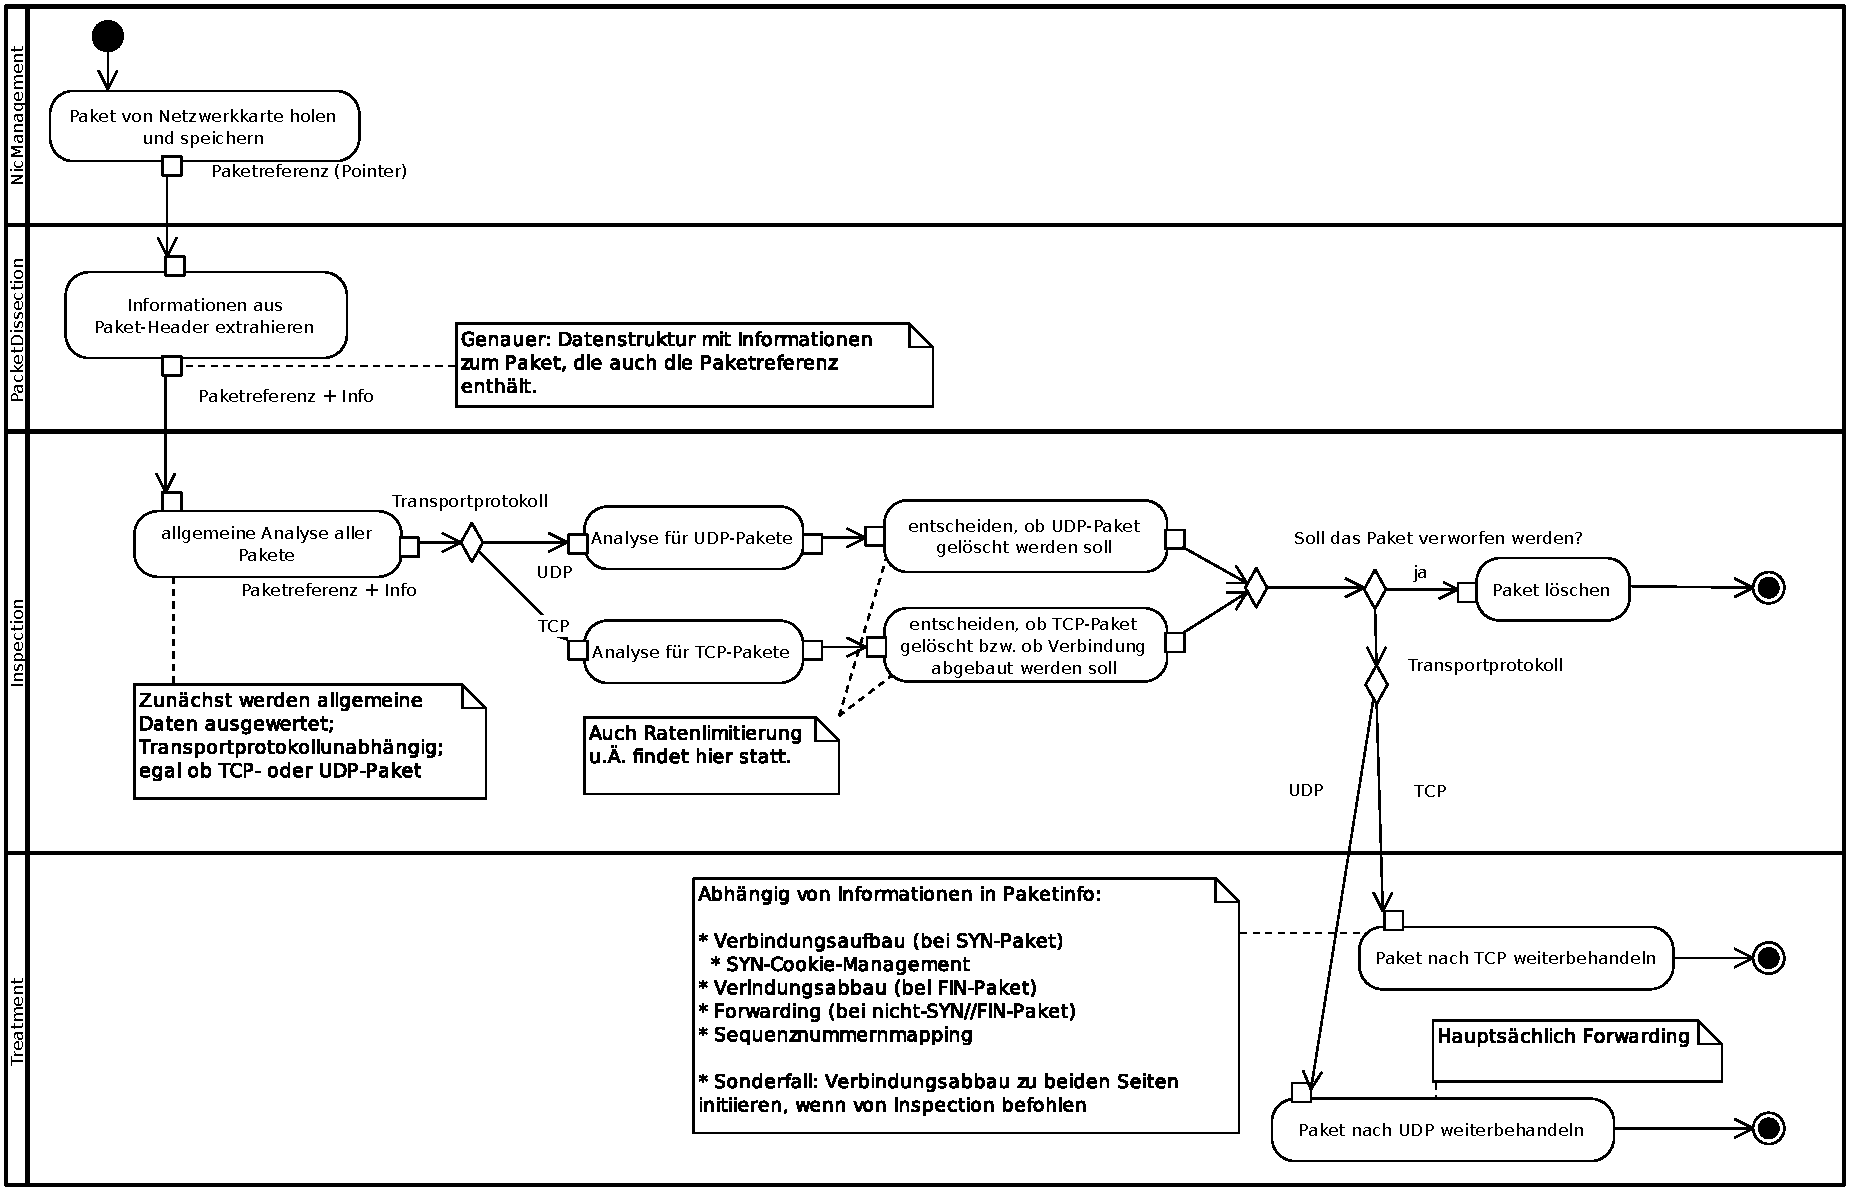
\includegraphics[angle=270, width=0.8\linewidth]{activity_control_flow.pdf}
	\caption{Schematische Darstellung des Kontrollflusses}
	\label{fig:control_flow}
\end{figure}
In diesem Abschnitt soll veranschaulicht werden, wie die Behandlung eines Paketes vom NicManagement bis zum Treatment erfolgt. Dabei werden die Pakete selbst als Akteure angesehen und noch nicht deren Klassen. Hinweis: Ein Thread soll später mehrere Pakete auf einmal durch die Pipeline führen. In diesem Diagramm wird zur Übersichtlichkeit jedoch nur der Fluss eines Paketes gezeigt. Dieser lässt sich dann einfach auf eine größere Menge von Paketen anwenden. Ein Aktivitätsdiagramm ist unter Abbildung \ref{fig:control_flow} am Ende der Sektion \ref{section:basic_structure} zu finden. Die Aktion ,,Paket nach TCP behandeln'' ist auf Abbildung \ref{fig:tcp_treatment_rough} genauer veranschaulicht.


\subsection{Einsatz von parallelen Threads}
Zunächst ist jedoch ein wichtiger Aspekt der Architektur hervorzuheben. Von der Mitigation-Box wird gefordert, eine hohe Paket- und Datenlast verarbeiten zu können. Das Hardwaresystem, auf welchem das zu entwickelnde Programm laufen wird, besitzt eine Multicore-CPU, d.h. das System ist in der Lage, Aufgaben aus unterschiedlichen Threads parallel zu bearbeiten. Dies hat das Potential, die Rechengeschwindigkeit zu vervielfachen und so die Bearbeitungszeit für jedes Paket zu verringern.

Dabei stellt sich die Frage, was die Threads im Programm genau tun. Es wäre zum Beispiel möglich, dass jeder Thread eine Aufgabe übernimmt, d.h. es gäbe einen Thread, der nur Daten analysiert oder einen Thread, der nur Paketinformationen extrahiert. Eine solche Aufteilung würde allerdings zu einem hohen Grad an Inter-Thread-Kommunikation führen. Diese ist nicht trivial und kann einen Großteil der verfügbaren Ressourcen benötigen, was den durch die Parallelisierung erzielten Gewinn wieder zunichte machen könnte. Um dieses Risiko zu vermeiden soll stattdessen jeder Thread die gesamte Pipeline durchlaufen. So ist kaum Inter-Thread-Kommunikation notwendig. Außerdem ist es dann verhältnismäßig einfach, den Entwurf skalierbar zu gestalten: Wenn ein Prozessor mit größerer Anzahl an Kernen verwendet werden würde, könnten mehr Pakete parallel bearbeitet werden ohne dass die Architektur geändert werden muss.


\subsubsection{Verwendung von Receive-Side-Scaling}
Ein weiterer grundlegender Vorteil ergibt sich durch das von der Netzwerkkarte und von DPDK unterstützte Receive Side Scaling (RSS), siehe Abbildung \ref{fig:Receive-Side-Scaling}: Ein auf einem Port eingehendes Paket wird einer von mehreren sogenannten RX-Queues zugeordnet. Eine RX-Queue gehört immer zu genau einem Netzwerkkartenport, ein Port kann mehrere RX-Queues besitzen. Kommen mehrere Pakete bei der Netzwerkkarte an, so ist die Zuordnung von Paketen eines Ports zu seinen RX-Queues gleich verteilt - alle RX-Queues sind gleich stark ausgelastet. Diese Zuordnung wird durch eine Hashfunktion umgesetzt, in die Source und Destination Port-Nummer und IP-Adresse einfließen. Das führt dazu, dass Pakete, die auf einem Port ankommen und einer bestimmten Verbindung zugehören immer wieder zu der selben RX-Queue dieses Ports zugeordnet werden.

Ferner besteht die Möglichkeit, Symmetric RSS einzusetzen. Dieser Mechanismus sorgt dafür, dass die Pakete, die auf dem einen Port der Netzwerkkarte ankommen nach genau dem selben Prinzip auf dessen RX-Queues aufgeteilt werden, wie die auf dem anderen Port ankommenden Pakete auf dessen RX-Queues. So ergeben sich Paare von RX-Queues, die jeweils immer Pakete von den gleichen Verbindungen beinhalten. Angenommen, die RX-Queues sind mit natürlichen Zahlen benannt und RX-Queue 3 auf Port 0 und RX-Queue 5 auf Port 1 sind ein korrespondierendes RX-Queue-Paar. Wenn nun ein Paket P, zugehörig einer Verbindung V auf RX-Queue 3, Port 0 ankommt, dann weiß man, dass Pakete, die auf Port 1 ankommen und der Verbindung V angehören immer auf RX-Queue 5, Port 1 landen.

Neben RX-Queues existieren auch TX-Queues (Tranceive-Queues), die ebenfalls zu einem bestimmten Port gehören. Darin befindliche Pakete werden von der Netzwerkkarte auf den entsprechenden Port geleitet und gesendet.

Auf Basis dieses Mechanismus sollen die Threads wie folgt organisiert werden: Einem Thread gehört ein Paar von korrespondierenden RX-Queues (auf verschiedenen Ports) und daneben eine TX-Queue auf dem einen und eine TX-Queue auf dem anderen Port. Das bringt einige Vorteile mit sich: Es müssen zwei Arten von Informationen entlang der Pipeline gespeichert, verarbeitet und gelesen werden: Informationen zu einer Verbindung und Analyseinformationen/Statistiken. Daher ist kaum Inter-Thread-Kommunikation nötig, weil alle Informationen zu einer Verbindung in Datenstrukturen gespeichert werden können, auf die nur genau der bearbeitende Thread Zugriff haben muss. Bei Analyseinformationen ist das leider nicht der Fall. Diese müssen zumindest teilweise global gespeichert werden. Hier bietet es sich an, einen Thread für das Management dieser globalen Informationen zu verwenden, der dann mit den restlichen Threads kommuniziert. So müssen zumindest nur mehrere Threads mit genau einem Thread Informationen austauschen und nicht alle Threads untereinander.

Im Falle eines Angriffes ist die Seite des Angreifers (entsprechender Port z.B. ,,Port 0'') viel stärker belastet, als die Seite des Servers (z.B. ,,Port 1''). Wegen der gleich verteilten Zuordnung des eingehenden Traffics auf die RX-Queues und weil ein Thread von RX-Queues von beiden Ports regelmäßig Pakete pollt, sind alle Threads gleichmäßig ausgelastet und können die Pakete bearbeiten. Ein günstiger Nebeneffekt bei DDOS-Angriffen ist, dass die Absenderadressen von Angriffspaketen oft sehr unterschiedlich sind. Das begünstigt die gleichmäßige Verteilung von Paketen auf RX-Queues.

\begin{figure}[t]
    \centering
    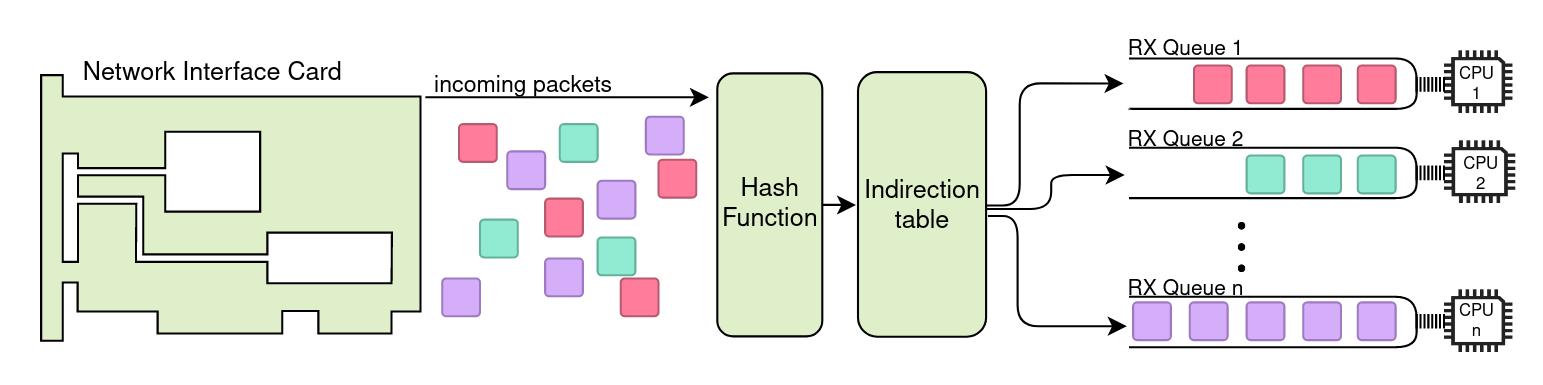
\includegraphics[width=0.95\linewidth]{Receive-Side-Scaling.png}
    \caption{Beispielhafte Paketverarbeitung mit Receive Side Scaling}
    \label{fig:Receive-Side-Scaling}
\end{figure}

\subsection{Paketdiagramm}
\begin{figure}[t]
    \centering
    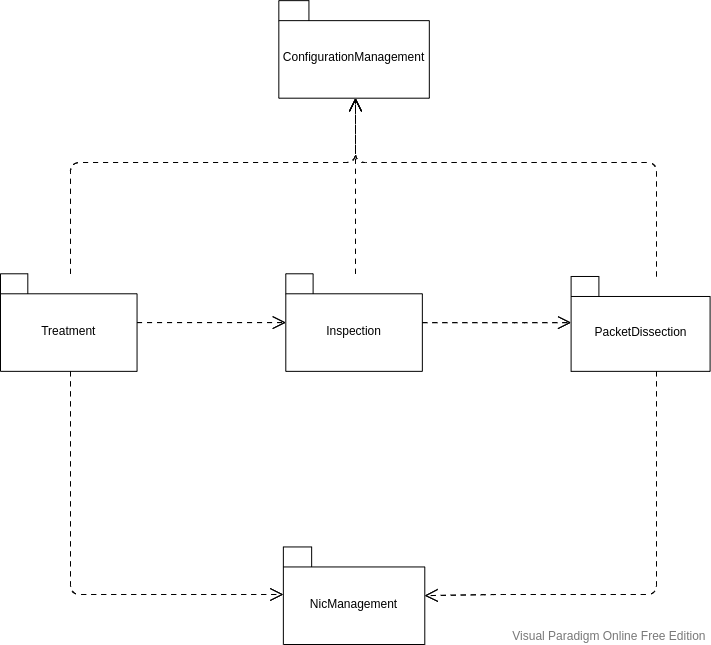
\includegraphics[width=0.7\linewidth]{DoS_Paketdiagramm}
    \caption{Paketdiagramm}
    \label{fig:dospaketdiagramm}
\end{figure}
Grundsätzlich ist es angedacht, wie im Paketdiagramm \ref{fig:dospaketdiagramm} ersichtlich, die zu entwickelnde Software in insgesamt 5 Teile zu untergliedern.

Das NicManagement wird eingesetzt, um die Kommunikation und Verwaltung der Netzwerkkarten und Ports zu ermöglichen, hier finden Operationen wie der Versand und Empfang von Paketen statt. Verwendet wird das NicManagement von der PacketDissection, welche ihrerseits dazu zuständig ist, die für die Erkennung und Klassifizierung von Angriffen benötigten, Informationen aus den einzelnen Headern eines Netzwerkpakets zu extrahieren. Die hieraus gewonnenen Informationen werden von der Inspection verwendet um sowohl Angriffe erkennen zu können, als auch über den allgemeinen Zustand des Systems in Form von Statistiken Auskunft zu geben. Das Treatment, welches sich um die Abwehrwehrmaßnahmen der verschiedenen Angriffe kümmert, verwendet hierzu die durch die Inspection bereitgestellten Ergebnisse und Informationen. Für das Versenden und Verwerfen von Pakten, sowie den Aufbau und das Terminieren von Verbindungen, verwendet das Treatment wiederum das NicManagement. Sowohl Treatment, als auch Inspection sowie PacketDissection verwenden den ConfigurationManagement, welches nicht nur die Aufgaben des Programmstarts übernimmt und für die Initialisierung sorgt, sondern auch wichtige Paramter für andere Programmbestandteile in Form von Konfigurationsdateien vorhält und einpflegt. Zudem ist das ConfigurationManagement die einzige Möglichkeit für den Nutzer, um aktiv Einstellungen am System vorzunehmen.

\subsection{Klassendiagramm}

Das Klassendiagramm untergliedert sich grundlegend in die selben Bestandteile wie das Paketdiagramm, siehe Bild \ref{fig:dospaketdiagramm}.

\subsubsection{NicManagement}
\begin{figure} [t]
	\centering
	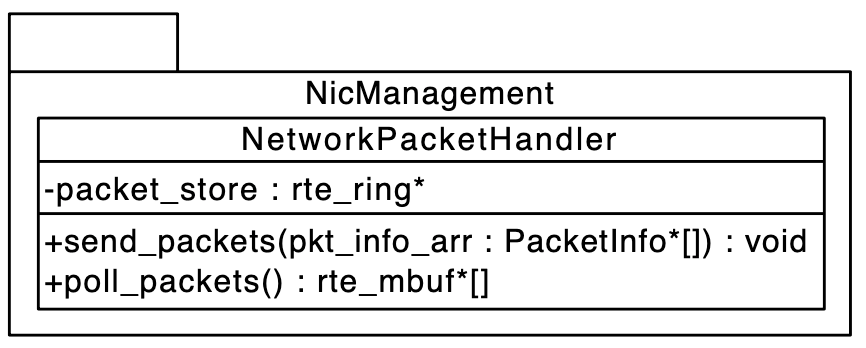
\includegraphics[width=0.6\linewidth]{package_NicManagement}
	\caption{Klasse NetworkPacketHandler im Package NicManagement}
	\label{fig:NetworkPacketHandler}
\end{figure}
Das NicManagement, siehe Abbildung \ref{fig:NetworkPacketHandler}, ist eine Abstraktion der Netzwerkkarte. Hier werden die Pakete von dem Interface gepollt und in den Speicher geschrieben. Um später mit diesen Paketen in anderen Paketen weiterarbeiten zu können, übergibt das NicManagement Pointer auf die Speicherbereiche, in denen sich die Pakete befinden. Der NetworkPacketHandler verwendet einen packet\_store rte-ring zum Abspeichern der empfangenen und zu versendenden Pakete.

Als Funktionalitäten stellt der NetworkPacketHandler sowohl send\_packets(pkt\_info\_arr:PacketInfo*[]) mit Rückgabetyp void, als auch poll\_packets() mit Rückgabetyp rte\_mbuf*[] bereit.

rte\_mbuf*[] in der Methode poll\_packets() steht für ein Array aus Pointern, die jeweils auf ein mbuf-Objekt zeigen. Hier ist nicht relevant, ob dies später auch wirklich als Array implementiert wird. Es soll vielmehr gezeigt werden, dass mehrere mbuf-Pointer auf einmal zurückgegeben werden.
\subsubsection{ConfigurationManagement}
\begin{figure} [t]
	\centering
	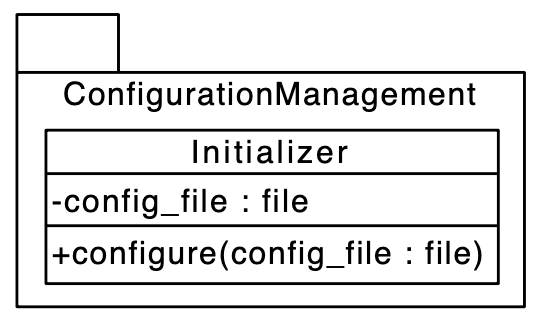
\includegraphics[width=0.5\linewidth]{package_ConfigurationManagement}
	\caption{Klasse Initializator im Package ConfigurationManagement}
	\label{fig:Initializator}
\end{figure}

Im Paket ConfigurationManagement, Abbildung \ref{fig:Initializator} findet die Initialisierung des Programms, sowie die Verwaltung der Konfigurationsdateien statt.

Als Attribut ist hier ausschließlich eine Konfigurationsdatei config\_file vom Typ conf vorgesehen.

Die Operationen beschränken sich auf configure(config\_file:file), wobei der Nutzer hier die Möglichkeit hat, über die Eingabe einer Konfigurationsdatei einzelne Parameter anzupassen.

\subsubsection{PacketDissection}
\begin{figure} [t]
	\centering
	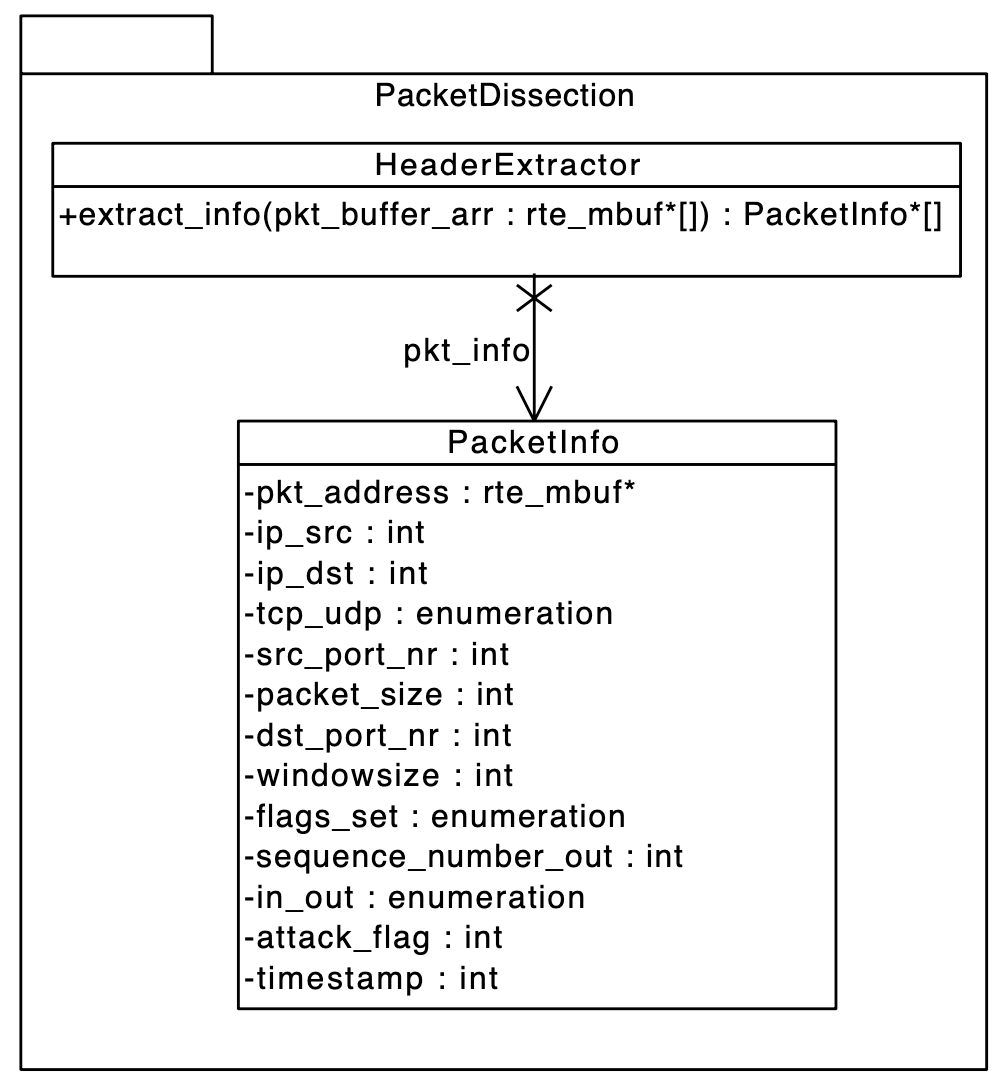
\includegraphics[width=0.7\linewidth]{package_PackageDissection}
	\caption{Klassen HeaderExtractor und PacketInfo im Package PackageDissection}
	\label{fig:HeaderExtractor}
\end{figure}
Die PacketDissection, Abbildung \ref{fig:HeaderExtractor} nimmt Pointer auf Pakete entgegen und extrahiert daraus die für die Erkennung und Behandlung wichtigen Headerinformationen. Weitergegeben werden dann Zeiger auf von der PacketDissection angelegte PacketInfo-Strukturen, genau eine für jedes Paket. Diese Struktur beinhaltet die extrahierten Informationen und den Pointer auf das zugehörige Paket, der vom NicManagement erhalten wurde.

Hierzu werden zwei Klassen verwendet, HeaderExtractor kümmert sich um das Extrahieren der Headerinformationen, PacketInfo wiederum wird als eigener Datentyp verwendet.

Die Klasse HeaderExtractor verwendet vorerst keinerlei Attribute und bietet nur die Methode
extract\_info(pkt\_buffer\_arr: rte\_mbuf*[]): PacketInfo*[] bereit, welche ihrerseits ein Array aus rte\_mbuf Pointern erhält und als Resultat ein Array aus PacketInfo Pointern zurückgibt.

Die Klasse PacketInfo ist als Kapselung mehrerer individueller Informationen aus den Netzwerkpaketen gedacht, hierunter fallen beispielsweise die Ziel-IP oder Paketgröße.


\subsubsection{Inspection}
\begin{figure} [t]
	\centering
	\includegraphics[width=0.6\linewidth]{package_inspection.pdf}
	\caption{Klassen StatisticsGenerator, Analyzer und StatInfo im Package Inspection}
		\label{fig:Inspection}
\end{figure}
Die Inspektion, siehe Abbildung \ref{fig:Inspection}, nimmt die bereitgestellten PacketInfo-Strukturen entgegen. Aus den beinhalteten Daten werden Statistiken und Regeln erstellt und ausgewertet. Gegebenenfalls sind manche Regeln dynamisch anzupassen.  In der Inspektion wird beurteilt, ob ein Paket legitim ist oder nicht. Ist es nicht legitim, wird es gelöscht. Wenn es nicht gelöscht wird, wird der Pointer auf die entsprechende PacketInfo-Struktur der Treatment-Komponente übergeben. Dieser Pointer ist die einzige Schnittstelle zwischen Inspektion und Treatment.

Weitere Anweisungen, wie mit dem Paket im Treatment verfahren werden soll können über die PacketInfo-Struktur mitgeteilt werden. Diese Möglichkeit wird genutzt, wenn eine TCP-Verbindung zu beiden Seiten abgebaut werden soll. Es wird eine entsprechende Direktive in die PacketInfo-Struktur geschrieben, die von der Treatment-Komponente ausgewertet wird.

Die Klasse Analyzer nutzt einen packet\_info\_buf vom Typ Patchmap zum Speichern der PacketInfo Daten, und enthält einen stat\_generator vom Typ StatisticsGenerator sowie statistics vom Typ StatInfo. Die Operation analyze(pkt\_info\_arr: PacketInfo*[]): PacketInfo*[] ist für die Verwaltung und den Aufruf aller weiterer detect-Methoden zuständig. Die jeweiligen detect-Methoden sollen je eine Angriffsart erkennen, und gegebenenfalls bereits erste, als schädlich erkannte Pakete mittels der drop\_packet-Methode verwerfen.

Die Klasse StatisticsGenerator ist für die Generierung von Statistiken zuständig, hierzu verwendet es einen packet\_info\_buf des Typs Patchmap, sowie eine Variable observed\_time, welche die bisher verstrichene Zeit speichert.
Die Operation generate\_statistic() wird dafür eingesetzt, Statistiken für die Analyse durch den Analyzer zu erstellen, sowie informative Daten für den Administrator zu erheben.
generate\_plot() erzeugt aus den ausgewerteten Daten anschauliche Diagramme, welche dem Administrator des Systems einen grundsätzlichen Überblick über den Zustand des Systems gewährt.
dump\_statistics() speichert die angefertigten Statistiken dann persistent auf dem System.

Die Klasse StatInfo dient als Speicherkonstrukt für die erhobenen Daten, welche beim Erzeugen und Auswerten einer Statistik anfallen.

Das Paket Inspection könnte, wenn nötig, außerdem eine Tabelle zu jeder Verbindung beinhalten (ähnlich der im TCP-Treatment). Aber es soll auf keinen Fall dieselbe Tabelle wie im TCP-Treatment genutzt werden, um die UML-Pakete zu kapseln.

\subsection{Treatment}
\begin{figure} [t]
	\centering
	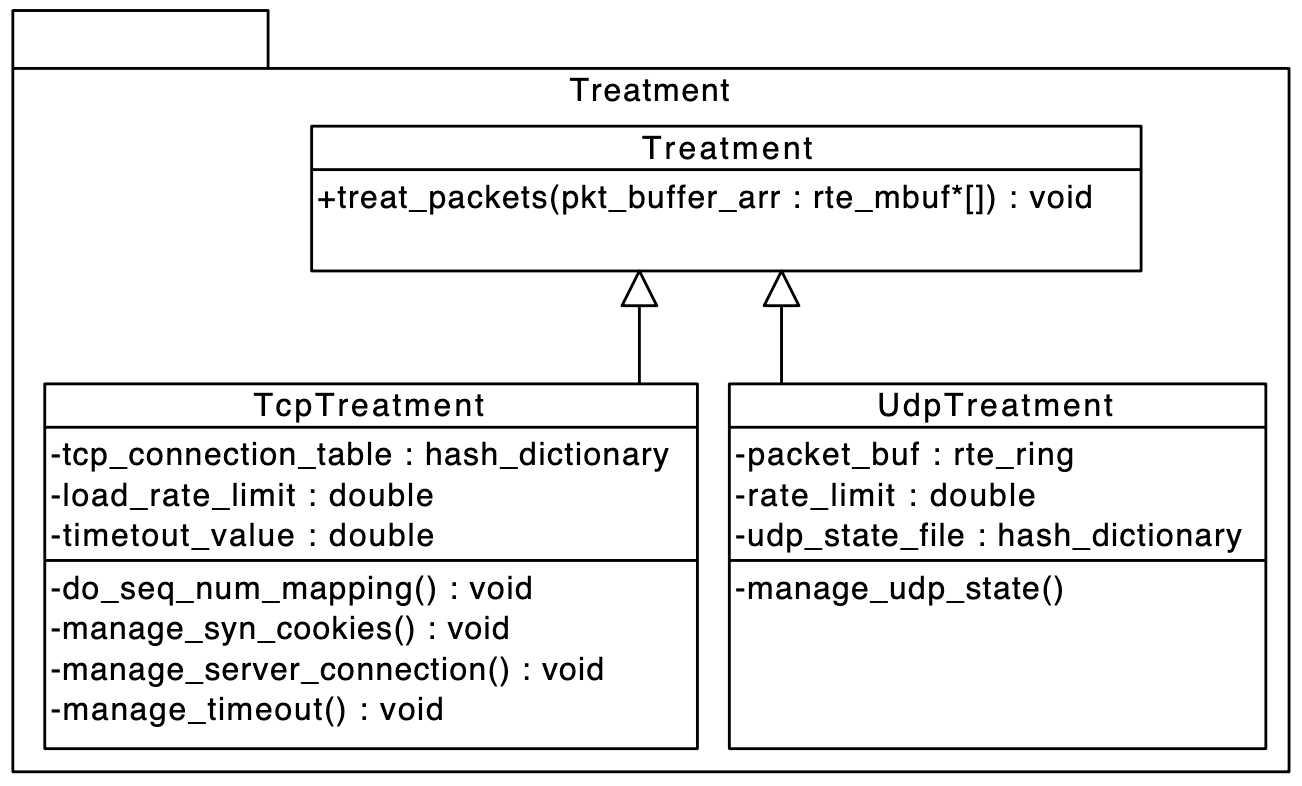
\includegraphics[width=0.6\linewidth]{package_Treatment}
	\caption{Klassen StatisticsGenerator, Analyzer und StatInfo im Package Inspection}
	\label{fig:Treatment}
\end{figure}
Das Paket Treatment, siehe Abbildung \ref{fig:Treatment}, hat zur Aufgabe, die zum Schutz der Server benötigten Operationen auszuführen. Hierbei werden zwei Klassen genutzt, wovon sich eine rein um die Behandlung von TCP-Paketen, eine andere nur um die Behandlung von UDP-Paketen vornimmt.
Das Treatment nimmt PacketInfo-Struktur-Pointer entgegen und behandelt das Paket nach dem entsprechende Transportprotokoll. 

Die Klasse TcpTreatment nutzt als Attribute eine tcp\_connection\_table vom Typ Hashmap, welche alle Informationen zu den einzelnen Verbindungen enthält, ein load\_rate\_limit des Typs double, sowie einen timeout\_value des Typs double.
Die Operation manage\_syn\_cookies() mit Rückgabetyp void erledigt jede, zur Verwaltung der SYN-Cookies benötigte, Aufgabe, wie das Berechnen des Hashwertes oder das Eintragen dieses in den Paketheader.
manage\_server\_connection() übernimmt alle Aufgaben, welche sich mit der Verwaltung der Verbindungen zu internen Servern befassen. Diese Methode wiederum verwendet die Methode do\_seq\_num\_mapping(), um die Verbindungen von externen Servern zur Middlebox, sowie die Verbindungen von internen Servern zur Middlebox zusammenzuführen.
Die Funktionen limit\_rate() und manage\_timeout() werden verwendet, um Angriffen wie TCP-Zero- und Small-Window-Angriffen entgegenzuwirken.

Die Klasse UdpTreatment hat einen packet\_buf des Typs rte\_ring, ein rate\_limit des Typs double, sowie ein udp\_state\_file des Typs hash\_dictionary als Attribute.
Als Funktionen stehen hier manage\_udp\_state zur Verfügung, welches aus dem eigentlich stateless UDP-Protokoll einen State zuweist. Des weiteren ist auch hier die Funktion limit\_rate() sowie manage\_timeout() verfügbar.

\section{Sequenzdiagramme}
    In folgendem Abschnitt finden sich Sequenzdiagramme, welche den genauen Ablauf der Behandlung verdeutlichen sollen. 
\subsection{SYN-FIN-ACK}
Abbildung \ref{fig:seqsynfinack} beschreibt den Ablauf der Erkennung und Behandlung eines SYN-FIN Angriffs. Zuerst erhält der Analyzer die Paketinformationen und überprüft diese auf Vorhandensein der Flagkombination, welche zur Detektion benötigt wird. Ist ein Paket als schädlich erkannt, so wird es bereits hier verworfen. 

\begin{figure}[t]
	\centering
	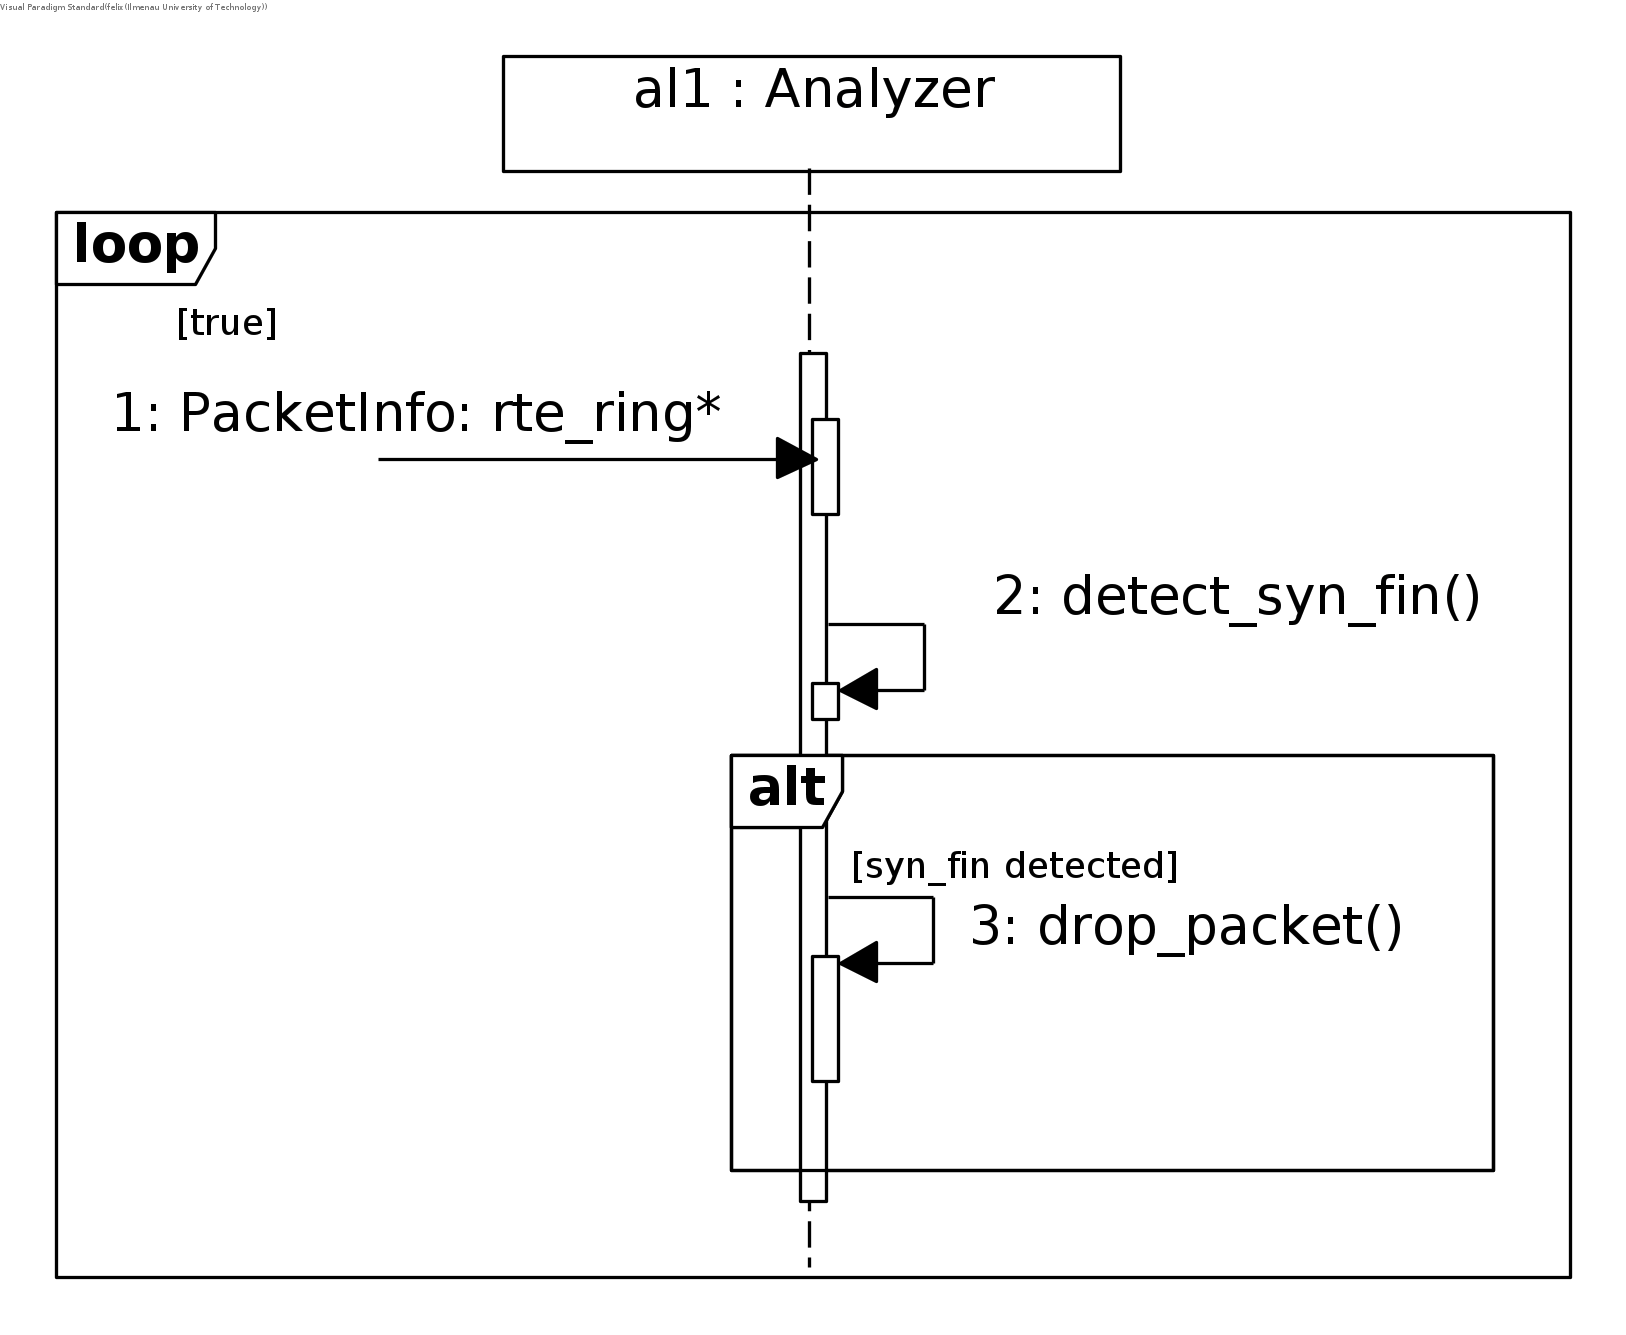
\includegraphics[width=0.5\linewidth]{Sequence_SYN-FIN-ACK}
	\caption{Sequenzdiagramm der SYN-FIN-ACK-Abwehr}
	\label{fig:seqsynfinack}
\end{figure}

\subsection{SYN-Flood}
Abbildung \ref{fig:sequencesyn-flood} beschreibt den Ablauf der Erkennung und Behandlung einer SYN-Flut. Zuerst erhält der Analyzer die Paketinformationen in Form eines rte\_ring Pointers. Die Funktion detect\_syn\_level() verwendet die dann vom StatisticsGenerator angeforderten StatInfos um das Level eines SYN-Angriffs zu informativen Zwecken zu berechnen. Es folgt die Übergabe der Packetinfos an das TCP-Treatment, welches seinerseits parallel das Management der SYN-Cookies sowie der internen Serververbindung vornimmt. Das Management der internen Serververbindungen selbst verwendet die Funktion do\_seq\_num\_mapping() um die Verbindungen zueinander führen zu können.

\begin{figure}[t]
    \centering
    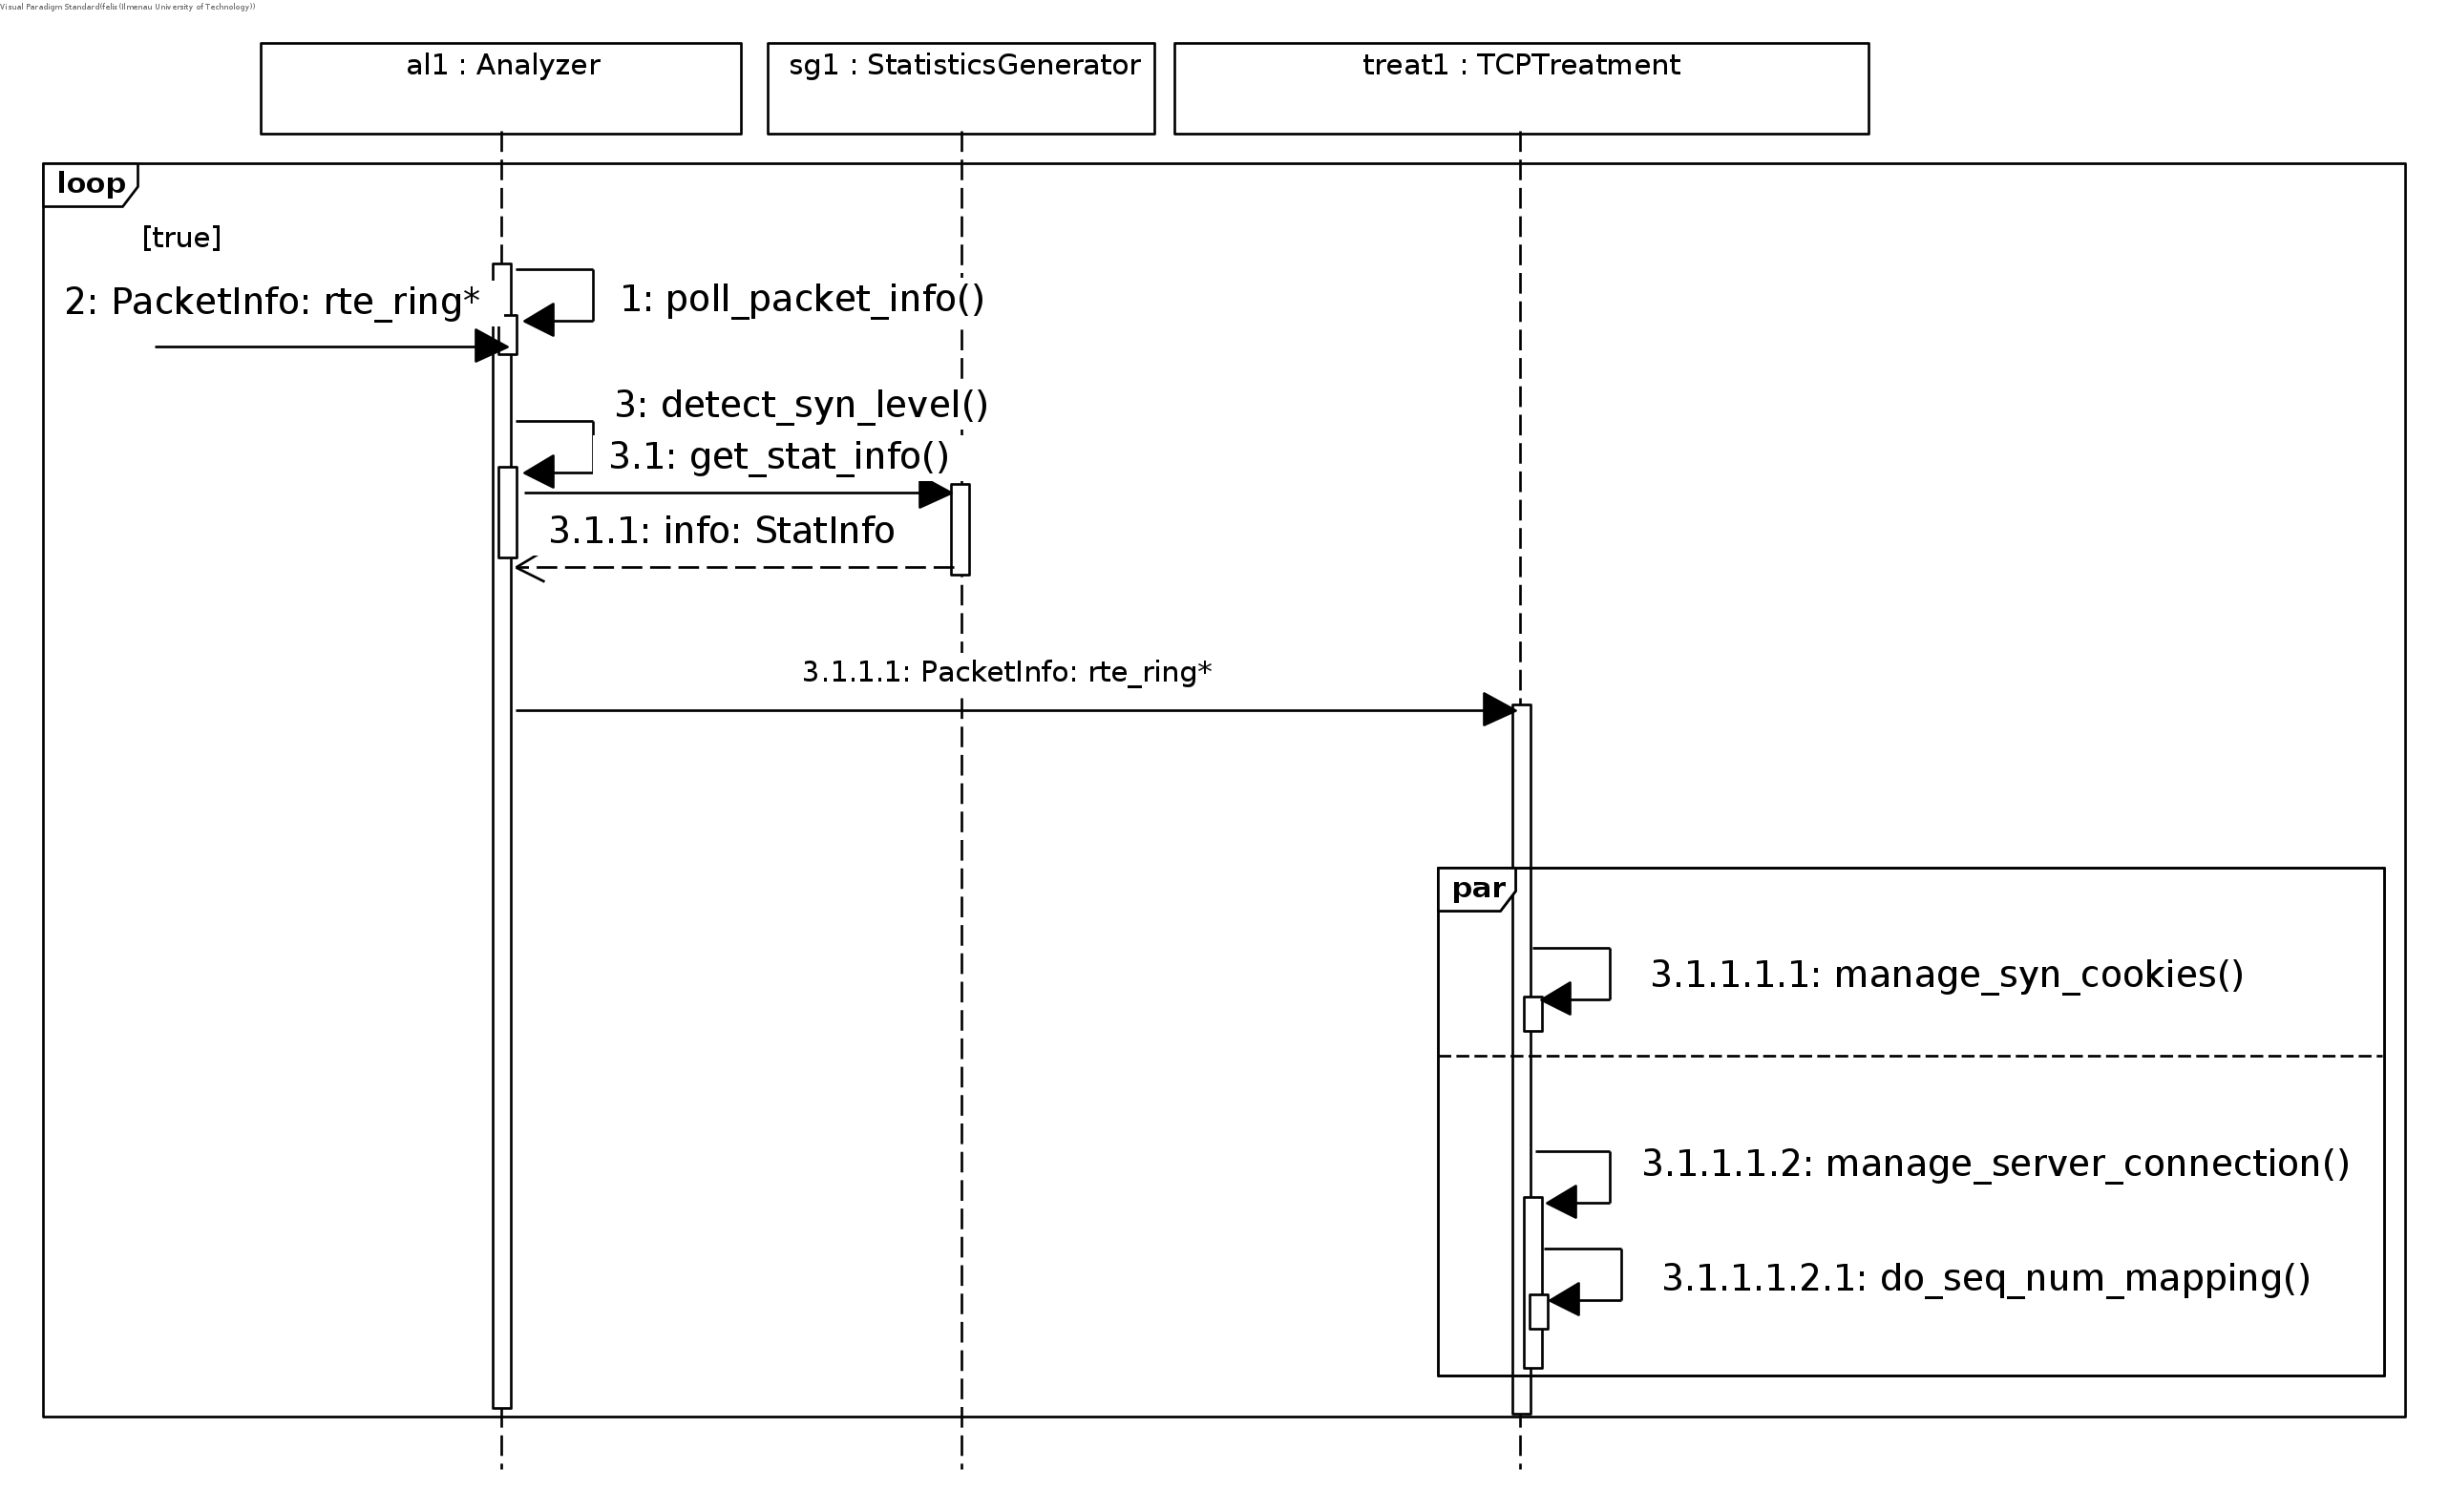
\includegraphics[width=0.95\linewidth]{Sequence_SYN-Flood}
    \caption{Sequenzdiagramm der SYN-Flood-Abwehr}
    \label{fig:sequencesyn-flood}
\end{figure}

\subsection{Small Windows}

Das Diagramm \ref{fig:sequence-smallwin} zeigt, wie das System Zero-Window- und Small-Window-Angriffe erkennt. Zunächst werden für eine Menge an Paketen die Methoden ,,detect\_zero\_window()'' und ,,detect\_small\_window()'' aufgerufen. Wenn ein Angriff erkannt wird, werden die entsprechenden Pakete verworfen. Danach werden alle gültigen Pakete zur normalen Weiterbehandlung and das Treatment weitergegeben.

\begin{figure}[t]
	\centering
	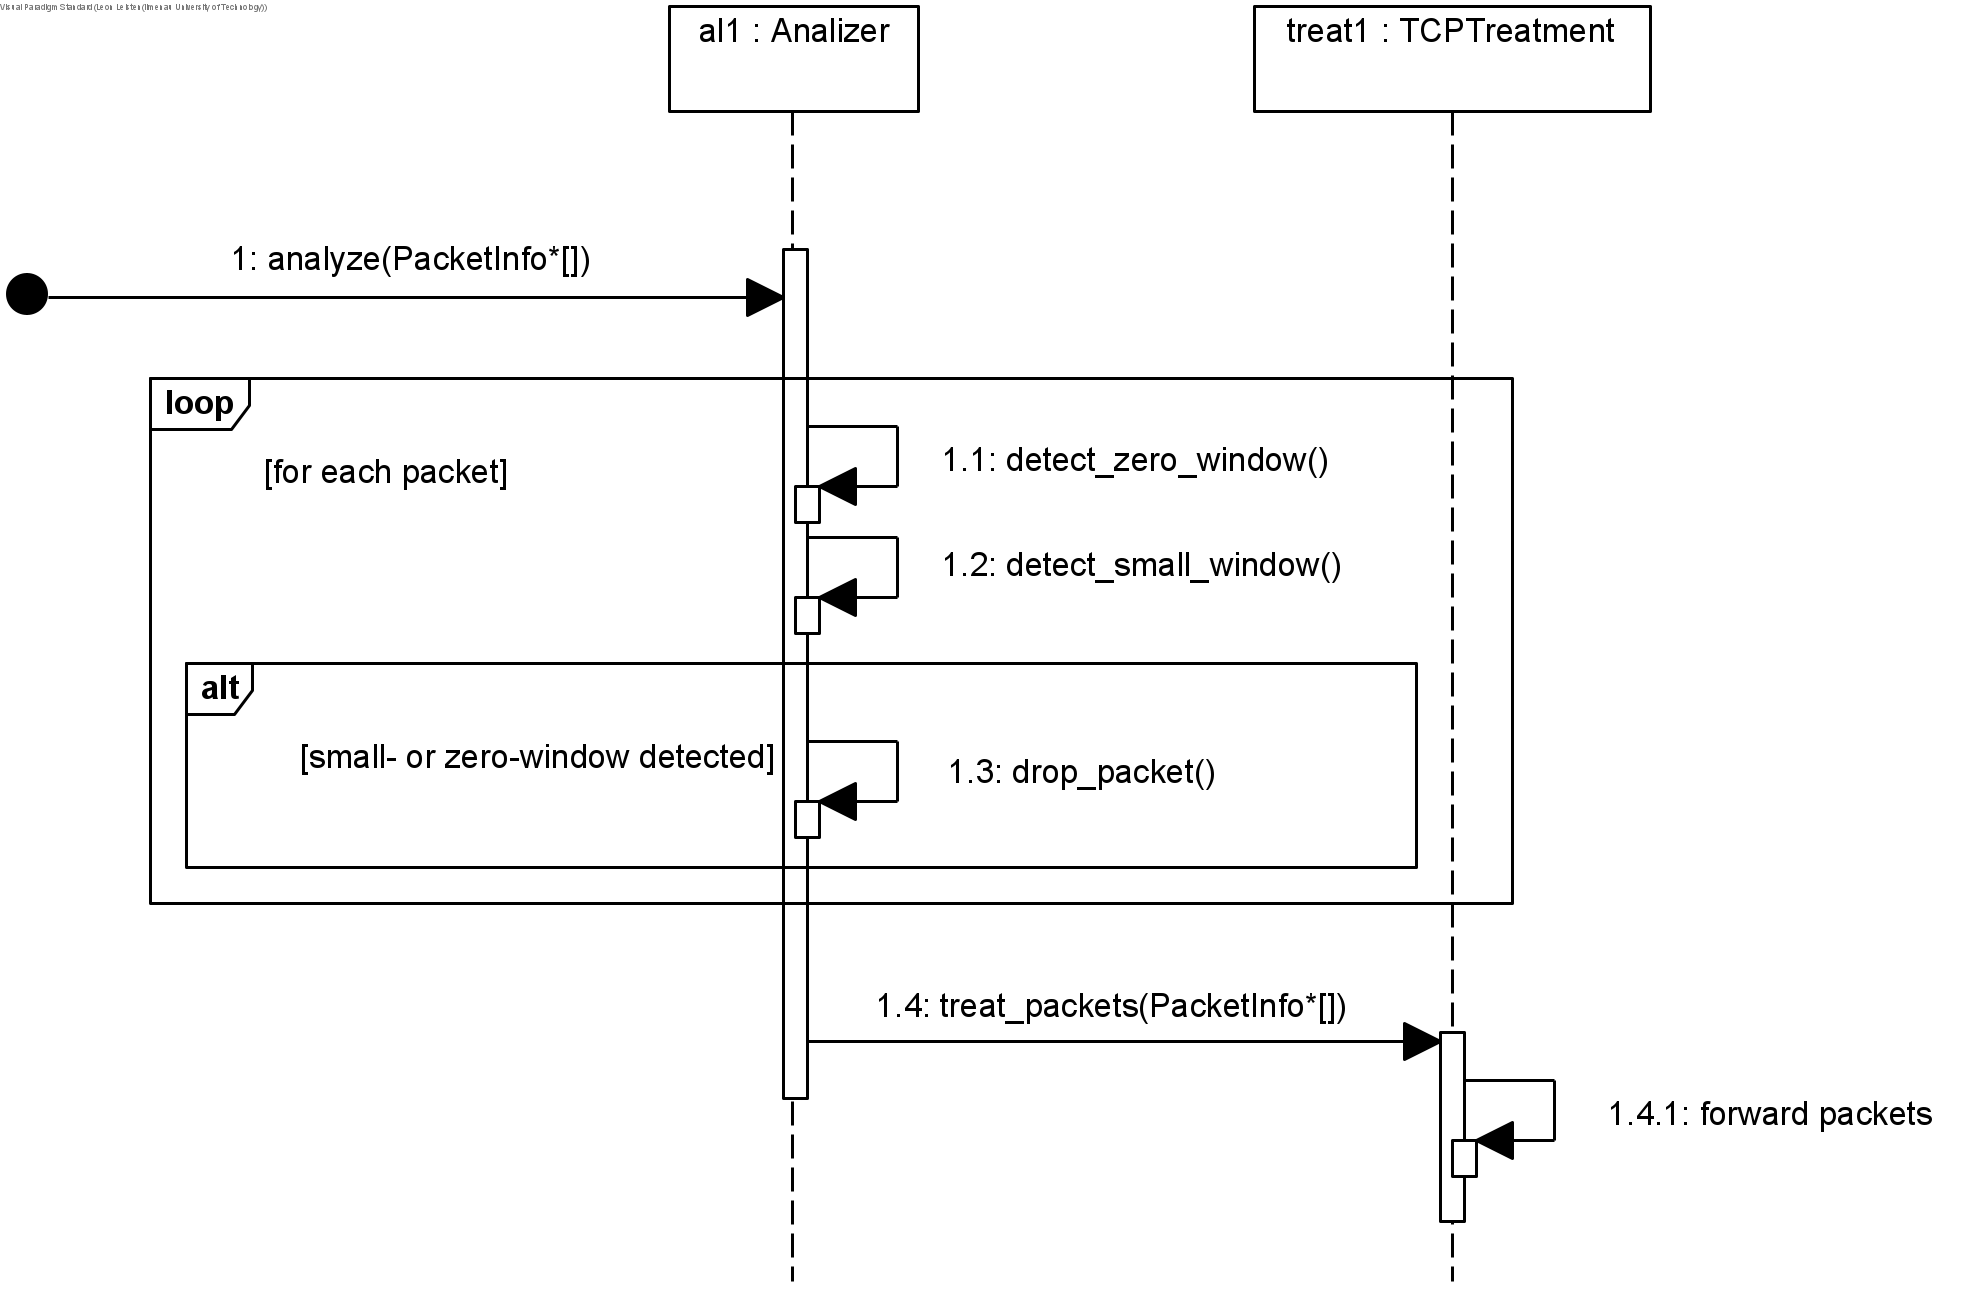
\includegraphics[width=0.8\textwidth]{zero-window__small-window_sequence_diagram.png}
	\caption{Sequenzdiagramm der Small-Window Abwehr}
	\label{fig:sequence-smallwin}
\end{figure}


\subsection{UDP Flood}
Bei der Abwehr eines UDP-Flood-Angriffes muss der Angriff zunächst erkannt werden, zu sehen in Abbildung \ref{fig:UDP-Flood-Erkennung}. Dies geschieht über die Methode ,,detect\_udp\_flood()''. Wird eine UDP-Flood erkannt, verwirft das Analyzer-Objekt das Paket, ansonsten wird dieses einem UdpTreatent-Objekt übergeben und gesendet.

\begin{figure}[t]
    \centering
    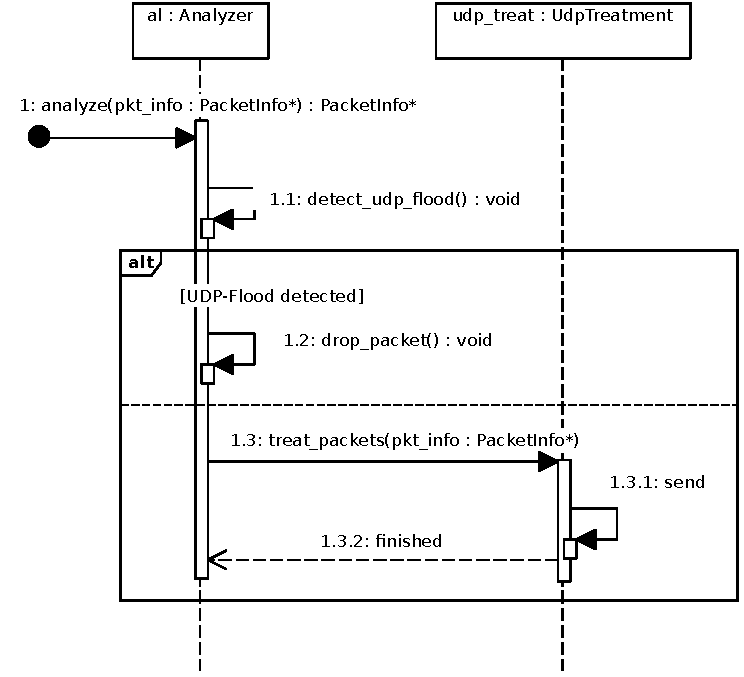
\includegraphics[width=0.7\linewidth]{sequence_udp_flood.pdf}
    \caption{Sequenzdiagramm der UDP-Flood-Erkennung}
    \label{fig:UDP-Flood-Erkennung}
\end{figure}

\end{document}

\section{Aktivitätsdiagramme}

\subsection{Behandlung eines Paketes nach TCP} \label{section:tcp_treat}
Unter Abbildung \ref{fig:tcp_treatment_rough} ist der Ablauf der Aktivität ,,Paket nach TCP behandeln'' zu finden. Die Idee hierbei ist, dass ein Paket-Pointer zusammen mit Informationen über das Paket, die sowohl aus dem Header extrahiert als auch von der Inspektion hinzugefügt wurden dem TcpTreatment übergeben wird. Das Paket wird dann anhand verschiedener Kriterien kategorisiert (SYN-Paket, ACK-Paket, FIN-Paket...) und infolgedessen entsprechend behandelt. Hier wird auch der SYN-Cookie-Mechanismus umgesetzt, welcher vor SYN-Flood-Attacken schützen soll.

Im Diagramm wird folgender Aufbau angenommen: A ist der Initiator eines Verbindungsauf- oder abbaus, B ist derjenige, der auf die Anfrage reagiert. M ist die Mitigation Box. Bei Verbindungsauf- und abbau ist also derjenige, der das erste SYN- bzw. FIN-Paket geschickt hat ,,A''. Der andere Kommunikationsteilnehmer ist demzufolge ,,B''. Hierbei wird nicht nach Angreifer und nicht-Angreifer unterschieden, es geht nur um die Kommunikation über TCP. Wenn bei einer Aktion ,,A<-M'' steht, bedeutet das, dass das die erwähnte Nachricht von M nach A geschickt wird. Wenn bei einem Pin (A->M) steht, bedeutet das, dass das entsprechende Paket von A gekommen ist.

Mit \textbf{,,initiales ACK''} ist das dritte Paket eines 3-Way-Handshakes gemeint, also das erste, das beim Verbindungsaufbau Nutzdaten enthält. \textbf{,,SN''} ist eine Abkürzung für ,,Sequenznummer''. \textbf{,,V-Tabelle''} steht für ,,Verbindungstabelle'', in einem Tupel stehen alle Daten zu genau einer Verbindung; zum Beispiel die Differenz der Sequenznummern von A und B für die Sequenznummerzuordnung. Das Wort ,,V-Tabelle'' ist nicht allgemein und ist nur eine Abkürzung. Im weiteren Entwurf soll diese Tabelle bzw. die entsprechende Datenstruktur einen passenden englischen Namen erhalten.

Um bestimmte Mechanismen auseinanderzuhalten werden zusammengehörige Aktionen farblich gekennzeichnet. \textbf{Grün} repräsentiert das Sequenznummermapping, \textbf{Hellgrün} das Zwischenspeichern und senden der Nutzdaten aus dem initialen ACK-Paket und \textbf{Cyan} das SYN-Cookie-Management.

\begin{figure}[t]
    \centering
    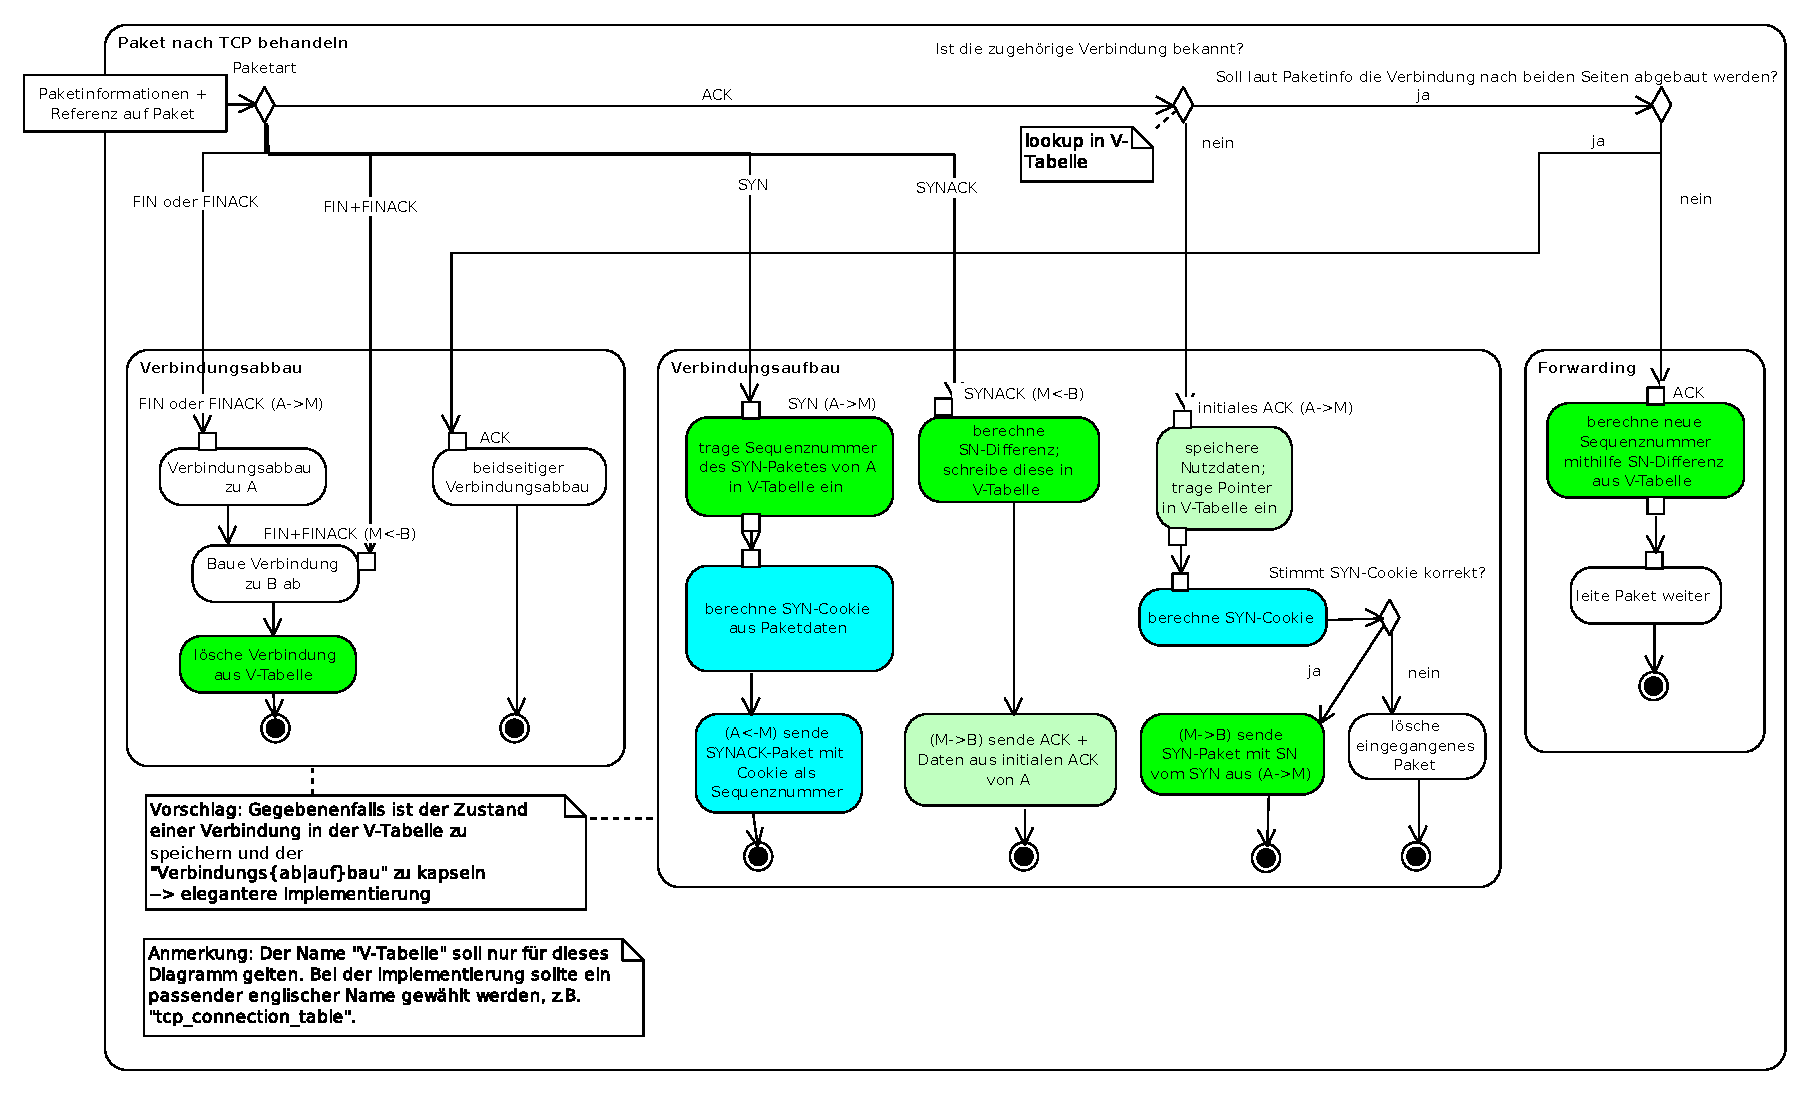
\includegraphics[angle=270, width=0.8\linewidth]{activity_tcp_treatment.pdf}
    \caption{Paketbehandlung nach TCP}
    \label{fig:tcp_treatment_rough}
\end{figure}






